\documentclass[8pt, handout]{beamer} 

%% Math packages
%%
\usepackage{amsmath,amsthm,amssymb}
% Removes the "Too many math alphabets used in version normal" error.
\newcommand\hmmax{0}
\newcommand\bmmax{0}
\usepackage[new]{old-arrows}
\usepackage{cancel}
\usepackage{mathdots}
\usepackage{venndiagram}
\usepackage{mathrsfs}          % Math script font

% Graphics
%%
\graphicspath{{./}{figs/}}
\usepackage{graphicx}
\usepackage{tikz}
\usetikzlibrary{arrows}
\usetikzlibrary{decorations.markings}
\usetikzlibrary{decorations.pathreplacing}
\usetikzlibrary{patterns}
\usetikzlibrary{shapes.geometric}
\usetikzlibrary{positioning}
\usetikzlibrary{matrix}
\usepackage{tikz-3dplot}
\usepackage{tkz-graph}
\usepackage{tikz-cd}

%% Colors 
%%
\usepackage{xcolor}
\usepackage{color}
\usepackage{visualalgebra}  %% Put this *after* the TikZ packages
\usepackage{visualalgebraslides}  %% Put this *after* "visualalgebra"

%% Page layout packages
%%
\usepackage{url}
\usepackage{multicol}
\usepackage{multirow}
\usepackage[numbers,square,sort&compress]{natbib}

%% Font and formatting packages
%%
\usepackage[english]{babel}    % Removing this causes compiler error
\usepackage{alltt}             % Like verbatim, but excludes \ and { }
\usepackage{enumerate}         % [shortlabels] option??
\usepackage{comment}
\usepackage{soul}              % strikeout text
\usepackage{bm}                % Bold math
\usepackage[T1]{fontenc}
\usepackage{relsize}

%% Fixes the \mathbf{} not working for fonts under 10pt
\usepackage{cmbright}
\fontencoding{OT1}\fontfamily{cmbr}\selectfont %to load ot1cmbr.fd
\DeclareFontShape{OT1}{cmbr}{bx}{n}{% change bx definition
<->cmbrbx10%
}{}
\normalfont

\makeatletter
\renewcommand*\env@matrix[1][\arraystretch]{%
  \edef\arraystretch{#1}%
  \hskip -\arraycolsep
  \let\@ifnextchar\new@ifnextchar
  \array{*\c@MaxMatrixCols c}}
\makeatother


%%=======================================================================

%% Beamer packages
%%
\mode<presentation>
{
  \usetheme{boadilla} 
  \useinnertheme{rectangles}
  \usecolortheme{dolphin}
}

\setbeamersize{text margin left=6mm}
\setbeamersize{text margin right=6mm}
\setbeamersize{sidebar width right=0mm}
\setbeamersize{sidebar width left=0mm}
\setbeamertemplate{navigation symbols}{}

\def\newblock{\hskip .11em plus .33em minus .07em}

% Other options: ball, circle, square 
\setbeamertemplate{enumerate items}[default]
%\setbeamercolor{enumerate subitem}{fg=red!80!black}
\def\opacity{0.5}
%\setbeamercovered{transparent}
\setbeamercovered{invisible}

\newcommand{\Pause}{\pause}      %% Comment this out => lots more page breaks


\AtBeginSection[]{
  \begin{frame}
  \vfill
  \centering
  \begin{beamercolorbox}[sep=8pt,center,shadow=true,rounded=true]{title}
    \usebeamerfont{title}\insertsectionhead\par%
  \end{beamercolorbox}
  \vfill
  \end{frame}
}

%%====================================================================

\title[Group actions, part 2!]{Group actions, part 2!}

\author[\href{mailto:sbagley@westminsteru.edu}{S. Bagley}]
       {\href{mailto:sbagley@westminsteru.edu}{Spencer Bagley}}

\institute[Westminster] { 
  \normalsize With many thanks to Matthew Macauley, \\
  \url{http://www.math.clemson.edu/~macaule/}}

\date[9 Apr 2025]{9 Apr 2025}

\begin{document}

\frame{\titlepage}

%%====================================================================

\begin{frame}{Overview} %\Pause

  Intuitively, a \Alert{group action} occurs when a group $G$
  ``naturally permutes'' a set $S$ \emph{of states}.

  \medskip\pause

  \begin{block}{Formal definition}
    A group $G$ \Alert{acts on} a set $S$ if there is a homomorphism
    $\phi\colon G\to\Perm(S)$. \pause

    We'll use \Alert{right group actions},
    
    and we'll write \Alert{$s.\phi(g)$} to denote ``where pushing the $g$-button sends state $s$.''
  \end{block} \pause

  \begin{block}{Definition}
    A set $S$ with a (right) action by $G$ is called a (right)
    \Alert{$G$-set}.
  \end{block} \pause
  
  \begin{alertblock}{Big ideas}
   \begin{itemize}
    \item An action $\phi\colon G\to\Perm(S)$ endows $S$ with an
      \textbf{algebraic structure}. \pause
    \item \emph{\Alert{Action graphs are to $G$-sets}, like how
      \Balert{Cayley graphs are to groups}.}
    \end{itemize}
  \end{alertblock}
  
\end{frame}

%%====================================================================

\begin{frame}{Five features of every group action} %\Pause

  Every group action has \textbf{five fundamental features} that we
  will always try to understand: \medskip\Pause

  \begin{tabular}{|l|l|l|}
    \hline
    & \Alert{local} (about an $s$ or a $g$)
    & \Palert{global} (about the whole action $\phi$)
    \\\hline
    subsets of $S$   & \begin{tabular}[c]{@{}l@{}}orbit of $s$\\ fixator of $g$\end{tabular} & fixed points of the action \\ \hline
    subgroups of $G$ & stabilizer of $s$                                                   & kernel of the action       \\ \hline
  \end{tabular}

  \medskip\Pause
  
  We will see parallels within and between these classes.
  
  \medskip\Pause
  
  For example, two ``local'' features will be ``dual'' to each
  other, as will the global features.

  \medskip\Pause
  
  Also, our global features can be expressed as intersections of our
  local features, either ranging over all $s\in S$, or over all $g\in
  G$.

  \medskip\Pause
  
  We'll start by exploring the three local features. \medskip\Pause

  \begin{exampleblock}{Notation}
    Throughout, we'll denote identity elements by $1\in G$ and $e\in\Perm(S)$.
  \end{exampleblock}

\end{frame}

%%====================================================================

\section{Local: orbits, stabilizers, fixators}

%%====================================================================

\begin{frame}{Two local features: orbits and stabilizers} %\Pause
  
  Suppose $G$ acts on set $S$, and pick some $s\in S$. We can ask two
  questions about it: \Pause
  
  \begin{enumerate}[(i)]
  \item What other \Alert{states} (in $S$) are reachable from $s$?
    (We call this the \Alert{orbit} of $s$.) \smallskip\Pause
  \item What {\color{xBlue}group elements} (in $G$) fix $s$?  (We
    call this the {\color{xBlue}stabilizer} of $s$.)
  \end{enumerate}
  
  \Pause
  
  \begin{block}{Definition}
    Suppose that $G$ acts on a set $S$ (on the right)
    via $\phi\colon G\to\Perm(S)$. \smallskip\Pause
    \begin{enumerate}[(i)]
    \item The \Alert{orbit} of $s\in S$ is the set 
      \[
      \orb(s)=\big\{s.\phi(g)\mid g\in G\big\}.
      \]
      \Pause\vspace{-5mm}
    \item The {\color{xBlue}stabilizer} of $s$ in $G$ is
      \[
      \stab(s)=\big\{g\in G\mid s.\phi(g)=s\big\}.
      \]
    \end{enumerate}
  \end{block}
  
  \Pause
  
  \begin{exampleblock}{In terms of the action graph}
    \begin{enumerate}[(i)]
    \item The \Alert{orbit} of $s\in S$ is the \Alert{connected
      component} containing $s$. \Pause
    \item The \Balert{stabilizer} of $s\in S$ are the group elements
      whose paths start and end at $s$; ``\Balert{loops}.''
    \end{enumerate}
  \end{exampleblock}
  
\end{frame}

%%====================================================================

\begin{frame}{The third local feature: fixators} %\Pause
  
  Our first two local features were specific to a certain element
  $s\in S$. \medskip\Pause

  Our last local feature is defined for each group element $g\in
  G$. \Pause A natural question to ask is:
  
  \begin{enumerate}
  \item[(iii)] What \emph{states} (in $S$) does $g$ fix?
  \end{enumerate}
  
  \Pause
  
  \begin{block}{Definition}
    Suppose that $G$ acts on a set $S$ (on the right)
    via $\phi\colon G\to\Perm(S)$.  \smallskip\Pause
    \begin{itemize}
    \item[(iii)] The \Galert{fixator} of $g\in G$ are       
      the elements $s\in S$ fixed by $g$:
      \[
      \fix(g)=\big\{s\in S\mid s\Dot\phi(g)=s\big\}.
      \]
    \end{itemize}
  \end{block}
  
  \Pause
  
  \begin{exampleblock}{In terms of the action graph}
    \begin{enumerate}
    \item[(iii)] The \Galert{fixator} of $g\in G$ are the nodes
      from which the $g$-paths are loops.
    \end{enumerate}
  \end{exampleblock}
  
  \Pause
  
  \begin{exampleblock}{In terms of the ``group switchboard analogy''}
    \begin{enumerate}[(i)]
    \item The \Alert{orbit} of $s\in S$ are the elements in $S$ the
      can be obtained by pressing some combination of buttons. \Pause
    \item The \Balert{stabilizer} of $s\in S$ consists of the buttons
      that have no effect on $s$. \Pause
    \item The \Galert{fixator} of $g\in G$ are the elements in
      $S$ that don't move when we press the $g$-button.
    \end{enumerate}
  \end{exampleblock}
  
\end{frame}

%%====================================================================

\begin{frame}{Three local features: orbits, stabilizers, and fixators}

  Here's the action graph of our running example of $D_4$ acting on $S$ the set of binary squares.

  \medskip

  Find the \Alert{orbit} and \Balert{stabilizer} of each binary square, and the \Galert{fixator} of each element of $D_4$.
  \[
  \scalebox{.85}{
    \begin{tikzpicture}[scale=.65,shorten >= -2pt, shorten <= -2pt]
      %%
      %% Group switchboard
      %%
      \begin{scope}[shift={(-9.25,-1.5)},scale=1]
        \tikzstyle{v} = [circle, draw, fill=lightgray,inner sep=0pt, 
          minimum size=5.4mm]
        %%
        \node at (.5,4) {\small \emph{``Group switchboard''}};
        \draw [midgray,fill=vYellow!50,rounded corners] (-.5,-.5)
        rectangle ++(2,4); 
        \node at (0,3) [v] {$1$}; \node at (1,3) [v,fill=vBlue] {$f$};
        \node at (0,2) [v,fill=vRed] {$r$}; \node at (1,2) [v] {$rf$};
        \node at (0,1) [v] {$r^2$}; \node at (1,1) [v] {$r^2\!f$};
        \node at (0,0) [v] {$r^3$}; \node at (1,0) [v] {$r^3\!f$};
      \end{scope}
      %%
      %% the size-1 orbit
      %%
      \begin{scope}[shift={(-5,0)},shorten >= 0pt, shorten <= 0pt]  
        \path[fill=actOrange] (-.5,0) rectangle ++(.5,.5); 
        \path[fill=actOrange] (0,0) rectangle ++(.5,.5);
        \path[fill=actOrange] (-.5,-.5) rectangle ++(.5,.5);
        \path[fill=actOrange] (0,-.5) rectangle ++(.5,.5);
        \draw (-.5,-.5) rectangle (.5,.5);
        \draw (-.25,.25) node{$0$}; \draw (.25,.25) node{$0$};
        \draw (-.25,-.25) node{$0$}; \draw (.25,-.25) node{$0$};
        \draw (-.5,-.5) rectangle (.5,.5);
        \Loop[dist=1.5cm,dir=NO,color=eRed](-.5,.5);
        \Loop[dist=1.5cm,dir=NO,color=eBlue](.5,.5);
      \end{scope}
      %%
      %% the size-2 orbit
      %%
      \begin{scope}[shift={(0,0)},shorten >= -2pt, shorten <= -2pt] 
        \begin{scope}[shift={(1.75,0)}]  %% H
          \path[fill=actPurple] (-.5,0) rectangle ++(.5,.5); 
          \path[fill=actOrange] (0,0) rectangle ++(.5,.5);
          \path[fill=actOrange] (-.5,-.5) rectangle ++(.5,.5);
          \path[fill=actPurple] (0,-.5) rectangle ++(.5,.5);
          \draw (-.5,-.5) rectangle (.5,.5);
          \draw (-.25,.25) node{$1$}; \draw (.25,.25) node{$0$};
          \draw (-.25,-.25) node{$0$}; \draw (.25,-.25) node{$1$};
          \node (0-out) at (-.5,.1) {};
          \node (0-in) at (-.5,-.1) {};
        \end{scope}
        %%
        \begin{scope}[shift={(-1.75,0)}] %% Hr^3
          \path[fill=actOrange] (-.5,0) rectangle ++(.5,.5); 
          \path[fill=actPurple] (0,0) rectangle ++(.5,.5);
          \path[fill=actPurple] (-.5,-.5) rectangle ++(.5,.5);
          \path[fill=actOrange] (0,-.5) rectangle ++(.5,.5);
          \draw (-.5,-.5) rectangle (.5,.5);
          \draw (-.25,.25) node{$0$}; \draw (.25,.25) node{$1$};
          \draw (-.25,-.25) node{$1$}; \draw (.25,-.25) node{$0$};
          \node (180-out) at (.5,-.1) {};
          \node (180-in) at (.5,.1) {};
        \end{scope}
        \draw [rr] (0-out) to [bend right=15] (180-in);
        \draw [bb] (180-out) to [bend right=15] (0-in);
      \end{scope} %% end of the size-2 orbit
      %%
      %% the size-4 orbit
      %%
      \begin{scope}[shift={(7,0)},shorten >= 0pt, shorten <= 0pt]  
        \begin{scope}[shift={(1.75,0)}]  %% H
          \path[fill=actOrange] (-.5,0) rectangle ++(.5,.5); 
          \path[fill=actOrange] (0,0) rectangle ++(.5,.5);
          \path[fill=actPurple] (-.5,-.5) rectangle ++(.5,.5);
          \path[fill=actPurple] (0,-.5) rectangle ++(.5,.5);
          \draw (-.5,-.5) rectangle (.5,.5);
          \draw (-.25,.25) node{$0$}; \draw (.25,.25) node{$0$};
          \draw (-.25,-.25) node{$1$}; \draw (.25,-.25) node{$1$};
          \node (0-out) at (0,.5) {};
          \node (0-in) at (0,-.5) {};
          \Loop[dist=1.5cm,dir=EA,color=eBlue](.5,0);
        \end{scope}
        %%
        \begin{scope}[shift={(0,1.75)}] %% Hr
          \path[fill=actOrange] (-.5,0) rectangle ++(.5,.5); 
          \path[fill=actPurple] (0,0) rectangle ++(.5,.5);
          \path[fill=actOrange] (-.5,-.5) rectangle ++(.5,.5);
          \path[fill=actPurple] (0,-.5) rectangle ++(.5,.5);
          \draw (-.5,-.5) rectangle (.5,.5);
          \draw (-.25,.25) node{$0$}; \draw (.25,.25) node{$1$};
          \draw (-.25,-.25) node{$0$}; \draw (.25,-.25) node{$1$};
          \node (90-out) at (-.5,0) {};
          \node (90-in) at (.5,0) {};
          \node (90-bb) at (0,-.5) {};
        \end{scope}
        %%
        \begin{scope}[shift={(-1.75,0)}] %% Hr^2
          \path[fill=actPurple] (-.5,0) rectangle ++(.5,.5); 
          \path[fill=actPurple] (0,0) rectangle ++(.5,.5);
          \path[fill=actOrange] (-.5,-.5) rectangle ++(.5,.5);
          \path[fill=actOrange] (0,-.5) rectangle ++(.5,.5);
          \draw (-.5,-.5) rectangle (.5,.5);
          \draw (-.25,.25) node{$1$}; \draw (.25,.25) node{$1$};
          \draw (-.25,-.25) node{$0$}; \draw (.25,-.25) node{$0$};
          \Loop[dist=1.5cm,dir=WE,color=eBlue](-.5,0);
          \node (180-out) at (0,-.5) {};
          \node (180-in) at (0,.5) {};
        \end{scope}
        %%
        \begin{scope}[shift={(0,-1.75)}] %% Hr^3
          \path[fill=actPurple] (-.5,0) rectangle ++(.5,.5); 
          \path[fill=actOrange] (0,0) rectangle ++(.5,.5);
          \path[fill=actPurple] (-.5,-.5) rectangle ++(.5,.5);
          \path[fill=actOrange] (0,-.5) rectangle ++(.5,.5);
          \draw (-.5,-.5) rectangle (.5,.5);
          \draw (-.25,.25) node{$1$}; \draw (.25,.25) node{$0$};
          \draw (-.25,-.25) node{$1$}; \draw (.25,-.25) node{$0$};        
          \node (270-out) at (.5,0) {};
          \node (270-in) at (-.5,0) {};
          \node (270-bb) at (0,.5) {};
        \end{scope}
        \draw [r,shorten >= -2pt, shorten <= -2pt] (0-out) to [bend right=25] (90-in);
        \draw [r,shorten >= -2pt, shorten <= -2pt] (90-out) to [bend right=25] (180-in);
        \draw [r,shorten >= -2pt, shorten <= -2pt] (180-out) to [bend right=25] (270-in);
        \draw [r,shorten >= -2pt, shorten <= -2pt] (270-out) to [bend right=25] (0-in);
        \draw [bb,shorten >= -2pt, shorten <= -2pt] (90-bb) to (270-bb);
      \end{scope} %% end of the size-4 orbit
  \end{tikzpicture}}
  \]
\end{frame}

%%====================================================================

\begin{frame}{Three local features: orbits, stabilizers, and fixators}
  \smallskip
  
  The \Alert{orbits} of our running example are the 3 connected
  components. \medskip
  
  Each node is labeled by its \Balert{stabilizer}.

  %% Action graph of D_4 = <r,f> acting on our 7 binary squares,
  %% labeled w/ stabilizers
  \[
  \scalebox{.85}{
    \begin{tikzpicture}[scale=.65,shorten >= -2pt, shorten <= -2pt]
      %%
      %% Group switchboard
      %%
      \begin{scope}[shift={(-9.25,-1.5)},scale=1]
        \tikzstyle{v} = [circle, draw, fill=lightgray,inner sep=0pt, 
          minimum size=5.4mm]
        %%
        \node at (.5,4) {\small \emph{``Group switchboard''}};
        \draw [midgray,fill=vYellow!50,rounded corners] (-.5,-.5)
        rectangle ++(2,4); 
        \node at (0,3) [v] {$1$}; \node at (1,3) [v,fill=vBlue] {$f$};
        \node at (0,2) [v,fill=vRed] {$r$}; \node at (1,2) [v] {$rf$};
        \node at (0,1) [v] {$r^2$}; \node at (1,1) [v] {$r^2\!f$};
        \node at (0,0) [v] {$r^3$}; \node at (1,0) [v] {$r^3\!f$};
      \end{scope}
      %%
      %% the size-1 orbit
      %%
      \begin{scope}[shift={(-5,0)},shorten >= 0pt, shorten <= 0pt]  
        \path[fill=actOrange] (-.5,0) rectangle ++(.5,.5); 
        \path[fill=actOrange] (0,0) rectangle ++(.5,.5);
        \path[fill=actOrange] (-.5,-.5) rectangle ++(.5,.5);
        \path[fill=actOrange] (0,-.5) rectangle ++(.5,.5);
        \draw (-.5,-.5) rectangle (.5,.5);
        \draw (-.25,.25) node{$0$}; \draw (.25,.25) node{$0$};
        \draw (-.25,-.25) node{$0$}; \draw (.25,-.25) node{$0$};
        \draw (-.5,-.5) rectangle (.5,.5);
        \Loop[dist=1.5cm,dir=NO,color=eRed](-.5,.5);
        \Loop[dist=1.5cm,dir=NO,color=eBlue](.5,.5);
        \node at (0,-1.2) {\normalsize $\bm{D_4\!=\!\<\Alert{r},\Balert{f}\>}$};
      \end{scope}
      %%
      %% the size-2 orbit
      %%
      \begin{scope}[shift={(0,0)},shorten >= -2pt, shorten <= -2pt] 
        \begin{scope}[shift={(1.75,0)}]  %% H
          \path[fill=actPurple] (-.5,0) rectangle ++(.5,.5); 
          \path[fill=actOrange] (0,0) rectangle ++(.5,.5);
          \path[fill=actOrange] (-.5,-.5) rectangle ++(.5,.5);
          \path[fill=actPurple] (0,-.5) rectangle ++(.5,.5);
          \draw (-.5,-.5) rectangle (.5,.5);
          \draw (-.25,.25) node{$1$}; \draw (.25,.25) node{$0$};
          \draw (-.25,-.25) node{$0$}; \draw (.25,-.25) node{$1$};
          \node (0-out) at (-.5,.1) {};
          \node (0-in) at (-.5,-.1) {};
          \node at (0,-1.2) {\normalsize $\bm{\<r^2,rf\>}$};
        \end{scope}
        %%
        \begin{scope}[shift={(-1.75,0)}] %% Hr^3
          \path[fill=actOrange] (-.5,0) rectangle ++(.5,.5); 
          \path[fill=actPurple] (0,0) rectangle ++(.5,.5);
          \path[fill=actPurple] (-.5,-.5) rectangle ++(.5,.5);
          \path[fill=actOrange] (0,-.5) rectangle ++(.5,.5);
          \draw (-.5,-.5) rectangle (.5,.5);
          \draw (-.25,.25) node{$0$}; \draw (.25,.25) node{$1$};
          \draw (-.25,-.25) node{$1$}; \draw (.25,-.25) node{$0$};
          \node (180-out) at (.5,-.1) {};
          \node (180-in) at (.5,.1) {};
          \node at (0,-1.2) {\normalsize $\bm{\<r^2,rf\>}$};
        \end{scope}
        \draw [rr] (0-out) to [bend right=15] (180-in);
        \draw [bb] (180-out) to [bend right=15] (0-in);
      \end{scope} %% end of the size-2 orbit
      %%
      %% the size-4 orbit
      %%
      \begin{scope}[shift={(7,0)},shorten >= 0pt, shorten <= 0pt]  
        \begin{scope}[shift={(1.75,0)}]  %% H
          \path[fill=actOrange] (-.5,0) rectangle ++(.5,.5); 
          \path[fill=actOrange] (0,0) rectangle ++(.5,.5);
          \path[fill=actPurple] (-.5,-.5) rectangle ++(.5,.5);
          \path[fill=actPurple] (0,-.5) rectangle ++(.5,.5);
          \draw (-.5,-.5) rectangle (.5,.5);
          \draw (-.25,.25) node{$0$}; \draw (.25,.25) node{$0$};
          \draw (-.25,-.25) node{$1$}; \draw (.25,-.25) node{$1$};
          \node (0-out) at (0,.5) {};
          \node (0-in) at (0,-.5) {};
          \Loop[dist=1.5cm,dir=EA,color=eBlue](.5,0);
          \node at (.9,.9) {\normalsize $\bm{\<f\>}$};
        \end{scope}
        %%
        \begin{scope}[shift={(0,1.75)}] %% Hr
          \path[fill=actOrange] (-.5,0) rectangle ++(.5,.5); 
          \path[fill=actPurple] (0,0) rectangle ++(.5,.5);
          \path[fill=actOrange] (-.5,-.5) rectangle ++(.5,.5);
          \path[fill=actPurple] (0,-.5) rectangle ++(.5,.5);
          \draw (-.5,-.5) rectangle (.5,.5);
          \draw (-.25,.25) node{$0$}; \draw (.25,.25) node{$1$};
          \draw (-.25,-.25) node{$0$}; \draw (.25,-.25) node{$1$};
          \node (90-out) at (-.5,0) {};
          \node (90-in) at (.5,0) {};
          \node (90-bb) at (0,-.5) {};
          \node at (-1.3,.5) {\normalsize $\bm{\<r^2f\>}$};
        \end{scope}
        %%
        \begin{scope}[shift={(-1.75,0)}] %% Hr^2
          \path[fill=actPurple] (-.5,0) rectangle ++(.5,.5); 
          \path[fill=actPurple] (0,0) rectangle ++(.5,.5);
          \path[fill=actOrange] (-.5,-.5) rectangle ++(.5,.5);
          \path[fill=actOrange] (0,-.5) rectangle ++(.5,.5);
          \draw (-.5,-.5) rectangle (.5,.5);
          \draw (-.25,.25) node{$1$}; \draw (.25,.25) node{$1$};
          \draw (-.25,-.25) node{$0$}; \draw (.25,-.25) node{$0$};
          \Loop[dist=1.5cm,dir=WE,color=eBlue](-.5,0);
          \node (180-out) at (0,-.5) {};
          \node (180-in) at (0,.5) {};
          \node at (-1.1,-1) {\normalsize $\bm{\<f\>}$};
        \end{scope}
        %%
        \begin{scope}[shift={(0,-1.75)}] %% Hr^3
          \path[fill=actPurple] (-.5,0) rectangle ++(.5,.5); 
          \path[fill=actOrange] (0,0) rectangle ++(.5,.5);
          \path[fill=actPurple] (-.5,-.5) rectangle ++(.5,.5);
          \path[fill=actOrange] (0,-.5) rectangle ++(.5,.5);
          \draw (-.5,-.5) rectangle (.5,.5);
          \draw (-.25,.25) node{$1$}; \draw (.25,.25) node{$0$};
          \draw (-.25,-.25) node{$1$}; \draw (.25,-.25) node{$0$};        
          \node (270-out) at (.5,0) {};
          \node (270-in) at (-.5,0) {};
          \node (270-bb) at (0,.5) {};
          \node at (1.2,-.5) {\normalsize $\bm{\<r^2f\>}$};
        \end{scope}
        \draw [r,shorten >= -2pt, shorten <= -2pt] (0-out) to [bend right=25] (90-in);
        \draw [r,shorten >= -2pt, shorten <= -2pt] (90-out) to [bend right=25] (180-in);
        \draw [r,shorten >= -2pt, shorten <= -2pt] (180-out) to [bend right=25] (270-in);
        \draw [r,shorten >= -2pt, shorten <= -2pt] (270-out) to [bend right=25] (0-in);
        \draw [bb,shorten >= -2pt, shorten <= -2pt] (90-bb) to (270-bb);
      \end{scope} %% end of the size-4 orbit
  \end{tikzpicture}}
  \]
  
  %% Fixators of elements in D_4, for our binary square example
  %%
  The \Galert{fixators} are $\fix(1)=S$, and
  \[
  \begin{tikzpicture}[scale=.5]
    \tikzstyle{every node}=[font=\scriptsize]
    %%
    \begin{scope}[shift={(0,0)}]
      \node at (-2.4,.5) {\normalsize $\fix(r)\!=\!\fix(r^3)\!=\!\Big\{$};
      \path[fill=actOrange] (0,.5) rectangle ++(.5,.5); 
      \path[fill=actOrange] (.5,.5) rectangle ++(.5,.5);
      \path[fill=actOrange] (0,0) rectangle ++(.5,.5);
      \path[fill=actOrange] (.5,0) rectangle ++(.5,.5);
      \draw (0,0) rectangle (1,1);
      \draw (.25,.75) node{$0$};\draw(.75,.75)node{$0$};
      \draw (.25,.25) node{$0$};\draw(.75,.25)node{$0$};
      \node at (1.3,.5) {$\Big\}$};
    \end{scope}
    %%
    \begin{scope}[shift={(11,0)}]
      \node at (-3.8,.5) {\normalsize
        $\fix(r^2)\!=\!\fix(rf)\!=\!\fix(r^3f)\!=\!\Big\{$};
      \path[fill=actOrange] (0,.5) rectangle ++(.5,.5); 
      \path[fill=actOrange] (.5,.5) rectangle ++(.5,.5);
      \path[fill=actOrange] (0,0) rectangle ++(.5,.5);
      \path[fill=actOrange] (.5,0) rectangle ++(.5,.5);
      \draw (0,0) rectangle (1,1);
      \draw (.25,.75) node{$0$};\draw(.75,.75)node{$0$};
      \draw (.25,.25) node{$0$};\draw(.75,.25)node{$0$};
      %%
      \node at (1.25,0) {$\Huge,$};
      %%
      \path[fill=actOrange] (1.5,.5) rectangle ++(.5,.5); 
      \path[fill=actPurple] (2,.5) rectangle ++(.5,.5);
      \path[fill=actPurple] (1.5,0) rectangle ++(.5,.5);
      \path[fill=actOrange] (2,0) rectangle ++(.5,.5);
      \draw (1.5,0) rectangle (2.5,1);
      \draw (1.75,.75) node{$0$};\draw(2.25,.75)node{$1$};
      \draw (1.75,.25) node{$1$};\draw(2.25,.25)node{$0$};
      %%
      \node at (2.75,0) {$\Huge,$};
      %%
      \path[fill=actPurple] (3,.5) rectangle ++(.5,.5); 
      \path[fill=actOrange] (3.5,.5) rectangle ++(.5,.5);
      \path[fill=actOrange] (3,0) rectangle ++(.5,.5);
      \path[fill=actPurple] (3.5,0) rectangle ++(.5,.5);
      \draw (3,0) rectangle (4,1);
      \draw (3.25,.75) node{$1$};\draw(3.75,.75)node{$0$};
      \draw (3.25,.25) node{$0$};\draw(3.75,.25)node{$1$};
      \node at (4.25,.5) {$\Big\}$};
      \end{scope}
    %%
    \begin{scope}[shift={(-.45,-1.75)}]
      \node at (-1.35,.5) {\normalsize $\fix(f)\!=\!\Big\{$};
      \path[fill=actOrange] (0,.5) rectangle ++(.5,.5); 
      \path[fill=actOrange] (.5,.5) rectangle ++(.5,.5);
      \path[fill=actOrange] (0,0) rectangle ++(.5,.5);
      \path[fill=actOrange] (.5,0) rectangle ++(.5,.5);
      \draw (0,0) rectangle (1,1);
      \draw (.25,.75) node{$0$};\draw(.75,.75)node{$0$};
      \draw (.25,.25) node{$0$};\draw(.75,.25)node{$0$};
      %%
      \node at (1.25,0) {$\Huge,$};
      %%
      \path[fill=actOrange] (1.5,.5) rectangle ++(.5,.5); 
      \path[fill=actOrange] (2,.5) rectangle ++(.5,.5);
      \path[fill=actPurple] (1.5,0) rectangle ++(.5,.5);
      \path[fill=actPurple] (2,0) rectangle ++(.5,.5);
      \draw (1.5,0) rectangle (2.5,1);
      \draw (1.75,.75) node{$0$};\draw(2.25,.75)node{$0$};
      \draw (1.75,.25) node{$1$};\draw(2.25,.25)node{$1$};
      %%
      \node at (2.75,0) {$\Huge,$};
      %%
      \path[fill=actPurple] (3,.5) rectangle ++(.5,.5); 
      \path[fill=actPurple] (3.5,.5) rectangle ++(.5,.5);
      \path[fill=actOrange] (3,0) rectangle ++(.5,.5);
      \path[fill=actOrange] (3.5,0) rectangle ++(.5,.5);
      \draw (3,0) rectangle (4,1);
      \draw (3.25,.75) node{$1$};\draw(3.75,.75)node{$1$};
      \draw (3.25,.25) node{$0$};\draw(3.75,.25)node{$0$};
      \node at (4.25,.5) {$\Big\}$};
    \end{scope}
    %%
    \begin{scope}[shift={(9,-1.75)}]
      \node at (-1.58,.5) {\normalsize $\fix(r^2f)\!=\!\Big\{$};
      \path[fill=actOrange] (0,.5) rectangle ++(.5,.5); 
      \path[fill=actOrange] (.5,.5) rectangle ++(.5,.5);
      \path[fill=actOrange] (0,0) rectangle ++(.5,.5);
      \path[fill=actOrange] (.5,0) rectangle ++(.5,.5);
      \draw (0,0) rectangle (1,1);
      \draw (.25,.75) node{$0$};\draw(.75,.75)node{$0$};
      \draw (.25,.25) node{$0$};\draw(.75,.25)node{$0$};
      %%
      \node at (1.25,0) {$\Huge,$};
      %%
      \path[fill=actOrange] (1.5,.5) rectangle ++(.5,.5); 
      \path[fill=actPurple] (2,.5) rectangle ++(.5,.5);
      \path[fill=actOrange] (1.5,0) rectangle ++(.5,.5);
      \path[fill=actPurple] (2,0) rectangle ++(.5,.5);
      \draw (1.5,0) rectangle (2.5,1);
      \draw (1.75,.75) node{$0$};\draw(2.25,.75)node{$1$};
      \draw (1.75,.25) node{$0$};\draw(2.25,.25)node{$1$};
      %%
      \node at (2.75,0) {$\Huge,$};
      %%
      \path[fill=actPurple] (3,.5) rectangle ++(.5,.5); 
      \path[fill=actOrange] (3.5,.5) rectangle ++(.5,.5);
      \path[fill=actPurple] (3,0) rectangle ++(.5,.5);
      \path[fill=actOrange] (3.5,0) rectangle ++(.5,.5);
      \draw (3,0) rectangle (4,1);
      \draw (3.25,.75) node{$1$};\draw(3.75,.75)node{$0$};
      \draw (3.25,.25) node{$1$};\draw(3.75,.25)node{$0$};
      \node at (4.25,.5) {$\Big\}$};
    \end{scope}
  \end{tikzpicture}
  \]

\end{frame}

%%====================================================================

\begin{frame}{Local duality: stabilizers vs.\ fixators} %\Pause

  Consider the following table, where a checkmark at $(g,s)$ means $g$
  fixes $s$. \vspace{-2mm}
  
  %% Fixed point table of our binary square example
  \[
  \renewcommand\arraystretch{1.8}
  \begin{tabular}{c|cccccccccccccc}
    && \begin{tikzpicture}[scale=.5]
         \tikzstyle{every node}=[font=\scriptsize]
         \path[fill=actOrange] (0,.5) rectangle ++(.5,.5); 
         \path[fill=actOrange] (.5,.5) rectangle ++(.5,.5);
         \path[fill=actOrange] (0,0) rectangle ++(.5,.5);
         \path[fill=actOrange] (.5,0) rectangle ++(.5,.5);
         \draw (.25,.75) node{$0$};\draw(.75,.75)node{$0$};
         \draw (.25,.25) node{$0$};\draw(.75,.25)node{$0$};
         \draw (0,0) rectangle (1,1); 
       \end{tikzpicture}
    && 
    \begin{tikzpicture}[scale=.5]
      \tikzstyle{every node}=[font=\scriptsize]
      \path[fill=actOrange] (0,.5) rectangle ++(.5,.5); 
      \path[fill=actPurple] (.5,.5) rectangle ++(.5,.5);
      \path[fill=actPurple] (0,0) rectangle ++(.5,.5);
      \path[fill=actOrange] (.5,0) rectangle ++(.5,.5);
      \draw (0,0) rectangle (1,1);
      \draw(.25,.75) node{$0$};\draw(.75,.75)node{$1$};
      \draw(.25,.25) node{$1$};\draw (.75,.25)node{$0$};
    \end{tikzpicture}
    &&
    \begin{tikzpicture}[scale=.5]
      \tikzstyle{every node}=[font=\scriptsize]
      \path[fill=actPurple] (3.5,.5) rectangle ++(.5,.5); 
      \path[fill=actOrange] (4,.5) rectangle ++(.5,.5);
      \path[fill=actOrange] (3.5,0) rectangle ++(.5,.5);
      \path[fill=actPurple] (4,0) rectangle ++(.5,.5);
      \draw (3.5,0) rectangle (4.5,1);
      \draw(3.75,.75) node{$1$};\draw(4.25,.75)node{$0$};
      \draw(3.75,.25) node{$0$};\draw (4.25,.25)node{$1$};
    \end{tikzpicture}
    &&
    \begin{tikzpicture}[scale=.5]
      \tikzstyle{every node}=[font=\scriptsize]
      \path[fill=actOrange] (0,.5) rectangle ++(.5,.5); 
      \path[fill=actOrange] (.5,.5) rectangle ++(.5,.5);
      \path[fill=actPurple] (0,0) rectangle ++(.5,.5);
      \path[fill=actPurple] (.5,0) rectangle ++(.5,.5);
      \draw (0,0) rectangle (1,1);
      \draw (.25,.75) node{$0$}; \draw (.75,.75) node{$0$};
      \draw (.25,.25) node{$1$}; \draw (.75,.25) node{$1$};
    \end{tikzpicture}
    &&
    \begin{tikzpicture}[scale=.5]
      \tikzstyle{every node}=[font=\scriptsize]
      \path[fill=actOrange] (0,.5) rectangle ++(.5,.5); 
      \path[fill=actPurple] (.5,.5) rectangle ++(.5,.5);
      \path[fill=actOrange] (0,0) rectangle ++(.5,.5);
      \path[fill=actPurple] (.5,0) rectangle ++(.5,.5);
      \draw (0,0) rectangle (1,1);
      \draw (.25,.75) node{$0$}; \draw (.75,.75) node{$1$};
      \draw (.25,.25) node{$0$}; \draw (.75,.25) node{$1$};
    \end{tikzpicture}
    &&
    \begin{tikzpicture}[scale=.5]
      \tikzstyle{every node}=[font=\scriptsize]
      \path[fill=actPurple] (0,.5) rectangle ++(.5,.5); 
      \path[fill=actPurple] (.5,.5) rectangle ++(.5,.5);
      \path[fill=actOrange] (0,0) rectangle ++(.5,.5);
      \path[fill=actOrange] (.5,0) rectangle ++(.5,.5);
      \draw (0,0) rectangle (1,1);
      \draw (.25,.75) node{$1$}; \draw (.75,.75) node{$1$};
      \draw (.25,.25) node{$0$}; \draw (.75,.25) node{$0$};
    \end{tikzpicture}
    &&
    \begin{tikzpicture}[scale=.5]
      \tikzstyle{every node}=[font=\scriptsize]
      \path[fill=actPurple] (0,.5) rectangle ++(.5,.5); 
      \path[fill=actOrange] (.5,.5) rectangle ++(.5,.5);
      \path[fill=actPurple] (0,0) rectangle ++(.5,.5);
      \path[fill=actOrange] (.5,0) rectangle ++(.5,.5);
      \draw (0,0) rectangle (1,1);
      \draw (.25,.75) node{$1$}; \draw (.75,.75) node{$0$};
      \draw (.25,.25) node{$1$}; \draw (.75,.25) node{$0$};
    \end{tikzpicture}
    \\ 
    \hline $1$ && \checkmark && \checkmark && \checkmark && \checkmark && \checkmark && \checkmark && \checkmark  \\
    $r$ && \checkmark && && && && && && \\
    $r^2$ && \checkmark && \checkmark && \checkmark && && && && \\
    $r^3$ && \checkmark && && && && && && \\
    $f$ && \checkmark && && && \checkmark && && \checkmark && \\
    $rf$ && \checkmark && \checkmark && \checkmark && && && && \\
    $r^2f$ && \checkmark && && && && \checkmark && && \checkmark \\
    $r^3f$ && \checkmark && \checkmark && \checkmark && && && && 
  \end{tabular}
  \]
  
  \Pause
  
  \begin{itemize}
  \item the \Balert{stablizers} can be read off the \Balert{columns}:
    \emph{group elements that \underline{fix} $s\in
      S$} \smallskip\Pause
  \item the \Galert{fixators} can be read off the \Galert{rows}:
    \emph{set elements \underline{fixed by} $g\in G$}.
  \end{itemize}
  
\end{frame}

%%====================================================================

\begin{frame}{The stabilizer subgroup} 

  Notice how in our example, the stabilizer of each $s\in S$ is a subgroup. 

  \medskip\Pause

  This holds true for any action. 
  
  \smallskip\Pause
  
  \begin{block}{Proposition}
    For any $s\in S$, the set $\stab(s)$ is a \Balert{subgroup} of $G$.
  \end{block}

  \Pause

  \begin{exampleblock}{Proof (outline)} %\Pause
    To show $\stab(s)$ is a group, we need to show three things: \Pause \\
    \begin{enumerate}[(i)]
    \item \textbf{Identity}. That is, $s.\phi(1)=s$. \Pause \\
    \item \textbf{Inverses}. \Pause That is, if $s.\phi(g)=s$, then
      $s.\phi(g^{-1})=s$. \Pause \\
    \item \textbf{Closure}. \Pause That is, if $s.\phi(g)=s$ and
      $s.\phi(h)=s$, then $s.\phi(gh)=s$. \Pause
    \end{enumerate}
    Alternatively, it suffices to show that if $s.\phi(g)=s$ and
    $s.\phi(h)=s$, then $s.\phi(gh^{-1})=s$, \medskip

    You'll do this on the homework.
  \end{exampleblock}

  \medskip\Pause
  
  All three of these are very intuitive in our our switchboard
  analogy.
 
\end{frame}

%%====================================================================

\begin{frame}[fragile]{The stabilizer subgroup}
  
  As we've seen, elements in the same orbit can have different stabilizers.

  \smallskip\Pause
  
  \begin{block}{Proposition (HW exercise)}
    Set elements in the same orbit have \Balert{conjugate stabilizers}:
    \[
    \stab(s\Dot\phi(g))=g^{-1}\stab(s)g,\quad\text{for all $g\in G$ and $s\in
    S$}.
    \] 
  \end{block}

  \smallskip\Pause
  
  In other words, if \Balert{$x$ stabilizes $s$}, then
  \Balert{$g^{-1}xg$ stabilizes $s.\phi(g)$}. \medskip\Pause

  Here are several ways to visualize what this means and why. \vspace{-3mm}
  
  %% Commutative diagram showing how elements in the same orbit have
  %% conjugate stabilizers
  \[
  \begin{tikzpicture}[scale=.375]
    \begin{scope}[shift={(-8.5,-3)}]
      \node at (0,0) {
        $\begin{tikzcd}[column sep=5.5em,row sep=4.5em]
          s \arrow[r,mapsto,"\phi(x)"] \arrow[d,mapsto,swap,"\phi(g)"]
          & s \arrow[d,mapsto,"\phi(g)"] \\   
          s' \arrow[r,mapsto,"\phi(g^{-1}xg)"] & s'
        \end{tikzcd}$};
    \end{scope}
    %%
    \tikzstyle{every node}=[font=\footnotesize]
    \begin{scope}[shift={(0,0)}]
      \path[fill=actOrange] (0,0) -- (0:1) -- (60:1) -- (0,0);
      \path[fill=actPurple] (0,0) -- (60:1) -- (120:1) -- (0,0);
      \path[fill=actOrange] (0,0) -- (120:1) -- (180:1) -- (0,0);
      \path[fill=actOrange] (0,0) -- (180:1) -- (240:1) -- (0,0);
      \path[fill=actOrange] (0,0) -- (240:1) -- (300:1) -- (0,0);
      \path[fill=actOrange] (0,0) -- (300:1) -- (0:1) -- (0,0);
      \node at (30:.6) {$0$}; \node at (90:.6) {$1$}; \node at (150:.6) {$0$};
      \node at (210:.6) {$0$}; \node at (270:.6) {$0$}; \node at (330:.6) {$0$};
      \draw (0:1) -- (60:1) -- (120:1) -- (180:1) -- (240:1) -- (300:1)--(0:1);
      \draw[-stealth'] (1.5,0) to node[midway,above] {\small$\phi(f)$} (7,0);
      \draw[-stealth'] (0,-1.5) to node[midway,left] {\small$\phi(r)$} (0,-4.5);
    \end{scope}
    %%
    \begin{scope}[shift={(8.5,0)}]
      \path[fill=actOrange] (0,0) -- (0:1) -- (60:1) -- (0,0);
      \path[fill=actPurple] (0,0) -- (60:1) -- (120:1) -- (0,0);
      \path[fill=actOrange] (0,0) -- (120:1) -- (180:1) -- (0,0);
      \path[fill=actOrange] (0,0) -- (180:1) -- (240:1) -- (0,0);
      \path[fill=actOrange] (0,0) -- (240:1) -- (300:1) -- (0,0);
      \path[fill=actOrange] (0,0) -- (300:1) -- (0:1) -- (0,0);
      \node at (30:.6) {$0$}; \node at (90:.6) {$1$}; \node at (150:.6) {$0$};
      \node at (210:.6) {$0$}; \node at (270:.6) {$0$}; \node at (330:.6) {$0$};
      \draw (0:1) -- (60:1) -- (120:1) -- (180:1) -- (240:1) -- (300:1) --(0:1);
      \draw[-stealth'] (0,-1.5) to node[midway,right] {\small$\phi(r)$}(0,-4.5);
    \end{scope}
    %%
    \begin{scope}[shift={(0,-6)}]
      \path[fill=actOrange] (0,0) -- (0:1) -- (60:1) -- (0,0);
      \path[fill=actOrange] (0,0) -- (60:1) -- (120:1) -- (0,0);
      \path[fill=actPurple] (0,0) -- (120:1) -- (180:1) -- (0,0);
      \path[fill=actOrange] (0,0) -- (180:1) -- (240:1) -- (0,0);
      \path[fill=actOrange] (0,0) -- (240:1) -- (300:1) -- (0,0);
      \path[fill=actOrange] (0,0) -- (300:1) -- (0:1) -- (0,0);
      \node at (30:.6) {$0$}; \node at (90:.6) {$0$}; \node at (150:.6) {$1$};
      \node at (210:.6) {$0$}; \node at (270:.6) {$0$}; \node at (330:.6) {$0$};
      \draw (0:1) -- (60:1) -- (120:1) -- (180:1) -- (240:1) -- (300:1) --(0:1);
      \draw[-stealth'] (1.5,0) to node[midway,above]
           {\small$\phi(r^{-1}fr)=\phi(r^4\!f)$} (7,0);
    \end{scope}
    %%
    \begin{scope}[shift={(8.5,-6)}]
      \path[fill=actOrange] (0,0) -- (0:1) -- (60:1) -- (0,0);
      \path[fill=actOrange] (0,0) -- (60:1) -- (120:1) -- (0,0);
      \path[fill=actPurple] (0,0) -- (120:1) -- (180:1) -- (0,0);
      \path[fill=actOrange] (0,0) -- (180:1) -- (240:1) -- (0,0);
      \path[fill=actOrange] (0,0) -- (240:1) -- (300:1) -- (0,0);
      \path[fill=actOrange] (0,0) -- (300:1) -- (0:1) -- (0,0);
      \node at (30:.6) {$0$}; \node at (90:.6) {$0$}; \node at (150:.6) {$1$};
      \node at (210:.6) {$0$}; \node at (270:.6) {$0$}; \node at (330:.6) {$0$};
      \draw (0:1) -- (60:1) -- (120:1) -- (180:1) -- (240:1) -- (300:1) --(0:1);
    \end{scope}
    %%
    \begin{scope}[shift={(14,.25)},scale=3]
      \tikzstyle{every node}=[font=\normalsize]
      \node[v] (s) at (0,-.5) {$s$};
      \path (s) edge [p,loop above,>=stealth] node[above] {$\Palert{x}$} (s);
      \node[v] (s') at (0,-2) {$s'$};
      \draw[g] (s) to node[midway,right] {$\Galert{g}$} (s');
    \end{scope}
  \end{tikzpicture}
  \]
  
  In other words, if \Palert{$x$} is a loop from $s$, and
  $s\stackrel{\Galert{g}}{\longto}s'$, then
  $\Galert{g^{-1}}\Palert{x}\Galert{g}$ is a loop from $s'$.
  
\end{frame}

%%====================================================================

\begin{frame}[fragile]{The stabilizer subgroup}
  
  Here is another example of an action (or $G$-set), this time of
  $G=D_6$ acting on these six ``Pacman hexagons.'' \bigskip

  Let $s$ be the highlighted hexagon, and $H=\stab(s)$. \medskip
  
  %% Size-6 orbit of D_6 action on hexagons, shown twice
  \[
  \hspace*{-3mm}
  \begin{tikzpicture}[scale=.48]
    %% The size-6 orbit
    \begin{scope}[shift={(0,0)},shorten >= -2pt, shorten <= -2pt]
      \begin{scope}[shift={(0:4)}, shorten >= 0pt, shorten <= 0pt] %% H
        \draw [yellow,rounded corners,fill=yellow] (0:1.3) -- (60:1.3) --
        (120:1.3) -- (180:1.3) -- (240:1.3) -- (300:1.3) -- (0:1.3);
        \path[fill=actOrange] (0,0) -- (0:1) -- (60:1) -- (0,0);
        \path[fill=actPurple] (0,0) -- (60:1) -- (120:1) -- (0,0);
        \path[fill=actOrange] (0,0) -- (120:1) -- (180:1) -- (0,0);
        \path[fill=actOrange] (0,0) -- (180:1) -- (240:1) -- (0,0);
        \path[fill=actOrange] (0,0) -- (240:1) -- (300:1) -- (0,0);
        \path[fill=actOrange] (0,0) -- (300:1) -- (0:1) -- (0,0);
        \draw (0:1) -- (60:1) -- (120:1) -- (180:1) -- (240:1)--(300:1)--(0:1);
        \node at (30:.6) {$0$};\node at (90:.6) {$1$};\node at (150:.6) {$0$};
        \node at (210:.6) {$0$};\node at (270:.6) {$0$};\node at (330:.6) {$0$};
        \node (0-out) at (90:.866) {};
        \node (0-in) at (270:.866) {};
        \node at (330:1.7) {$\bm{H}$};
        \Loop[dist=2cm,dir=NO,color=eBlue](.55,.866);
      \end{scope}
      %%
      \begin{scope}[shift={(60:4)}, shorten >= 0pt, shorten <= 0pt] %% Hr
        \path[fill=actOrange] (0,0) -- (0:1) -- (60:1) -- (0,0);
        \path[fill=actOrange] (0,0) -- (60:1) -- (120:1) -- (0,0);
        \path[fill=actPurple] (0,0) -- (120:1) -- (180:1) -- (0,0);
        \path[fill=actOrange] (0,0) -- (180:1) -- (240:1) -- (0,0);
        \path[fill=actOrange] (0,0) -- (240:1) -- (300:1) -- (0,0);
        \path[fill=actOrange] (0,0) -- (300:1) -- (0:1) -- (0,0);
        \draw (0:1) -- (60:1) -- (120:1) -- (180:1) -- (240:1)--(300:1)--(0:1);
        \node at (30:.6) {$0$};\node at (90:.6) {$0$};\node at (150:.6) {$1$};
        \node at (210:.6) {$0$};\node at (270:.6) {$0$};\node at (330:.6) {$0$};
        \node (60-out) at (150:.866) {};
        \node (60-in) at (330:.866) {};
        \node (60-bb) at (0,-.866) {};
        \node at (30:1.7) {$\bm{Hr}$};
      \end{scope}
      %%
      \begin{scope}[shift={(120:4)}, shorten >= 0pt, shorten <= 0pt] %% Hr^2
        \path[fill=actOrange] (0,0) -- (0:1) -- (60:1) -- (0,0);
        \path[fill=actOrange] (0,0) -- (60:1) -- (120:1) -- (0,0);
        \path[fill=actOrange] (0,0) -- (120:1) -- (180:1) -- (0,0);
        \path[fill=actPurple] (0,0) -- (180:1) -- (240:1) -- (0,0);
        \path[fill=actOrange] (0,0) -- (240:1) -- (300:1) -- (0,0);
        \path[fill=actOrange] (0,0) -- (300:1) -- (0:1) -- (0,0);
        \draw (0:1) -- (60:1) -- (120:1) -- (180:1) -- (240:1)--(300:1)--(0:1);
        \node at (30:.6) {$0$};\node at (90:.6) {$0$};\node at (150:.6) {$0$};
        \node at (210:.6) {$1$};\node at (270:.6) {$0$};\node at (330:.6) {$0$};
        \node (120-out) at (210:.866) {};
        \node (120-in) at (30:.866) {};
        \node (120-bb) at (0,-.866) {};
        \node at (150:1.7) {$\bm{Hr^2}$};
      \end{scope}
      %%
      \begin{scope}[shift={(180:4)}, shorten >= 0pt, shorten <= 0pt] %% Hr^3
        \path[fill=actOrange] (0,0) -- (0:1) -- (60:1) -- (0,0);
        \path[fill=actOrange] (0,0) -- (60:1) -- (120:1) -- (0,0);
        \path[fill=actOrange] (0,0) -- (120:1) -- (180:1) -- (0,0);
        \path[fill=actOrange] (0,0) -- (180:1) -- (240:1) -- (0,0);
        \path[fill=actPurple] (0,0) -- (240:1) -- (300:1) -- (0,0);
        \path[fill=actOrange] (0,0) -- (300:1) -- (0:1) -- (0,0);
        \draw (0:1) -- (60:1) -- (120:1) -- (180:1) -- (240:1)--(300:1)--(0:1);
        \node at (30:.6) {$0$};\node at (90:.6) {$0$};\node at (150:.6) {$0$};
        \node at (210:.6) {$0$};\node at (270:.6) {$1$};\node at (330:.6) {$0$};
        \node (180-out) at (270:.866) {};
        \node (180-in) at (90:.866) {};
        \node at (210:1.7) {$\bm{Hr^3}$};
        \Loop[dist=2cm,dir=NO,color=eBlue](-.55,.866);
      \end{scope}
      %%
      \begin{scope}[shift={(240:4)}, shorten >= 0pt, shorten <= 0pt] %% Hr^4
        \path[fill=actOrange] (0,0) -- (0:1) -- (60:1) -- (0,0);
        \path[fill=actOrange] (0,0) -- (60:1) -- (120:1) -- (0,0);
        \path[fill=actOrange] (0,0) -- (120:1) -- (180:1) -- (0,0);
        \path[fill=actOrange] (0,0) -- (180:1) -- (240:1) -- (0,0);
        \path[fill=actOrange] (0,0) -- (240:1) -- (300:1) -- (0,0);
        \path[fill=actPurple] (0,0) -- (300:1) -- (0:1) -- (0,0);
        \draw (0:1) -- (60:1) -- (120:1) -- (180:1) -- (240:1)--(300:1)--(0:1);
        \node at (30:.6) {$0$};\node at (90:.6) {$0$};\node at (150:.6) {$0$};
        \node at (210:.6) {$0$};\node at (270:.6) {$0$};\node at (330:.6) {$1$};
        \node (240-out) at (330:.866) {};
        \node (240-in) at (150:.866) {};
        \node (240-bb) at (0,.866) {};
        \node at (210:1.7) {$\bm{Hr^4}$};
      \end{scope}
      %%
      \begin{scope}[shift={(300:4)}, shorten >= 0pt, shorten <= 0pt]
        \path[fill=actPurple] (0,0) -- (0:1) -- (60:1) -- (0,0);
        \path[fill=actOrange] (0,0) -- (60:1) -- (120:1) -- (0,0);
        \path[fill=actOrange] (0,0) -- (120:1) -- (180:1) -- (0,0);
        \path[fill=actOrange] (0,0) -- (180:1) -- (240:1) -- (0,0);
        \path[fill=actOrange] (0,0) -- (240:1) -- (300:1) -- (0,0);
        \path[fill=actOrange] (0,0) -- (300:1) -- (0:1) -- (0,0);
        \draw (0:1) -- (60:1) -- (120:1) -- (180:1) -- (240:1)--(300:1)--(0:1);
        \node at (30:.6) {$1$};\node at (90:.6) {$0$};\node at (150:.6) {$0$};
        \node at (210:.6) {$0$};\node at (270:.6) {$0$};\node at (330:.6) {$0$};
        \node (300-out) at (30:.866) {};
        \node (300-in) at (210:.866) {};
        \node (300-bb) at (0,.866) {};
        \node at (330:1.7) {$\bm{Hr^5}$};
      \end{scope}
      %%
      \draw [r] (0-out) to [bend right=12] (60-in);
      \draw [r] (60-out) to [bend right=12] (120-in);
      \draw [r] (120-out) to [bend right=12] (180-in);
      \draw [r] (180-out) to [bend right=12] (240-in);
      \draw [r] (240-out) to [bend right=12] (300-in);
      \draw [r] (300-out) to [bend right=12] (0-in);
      \draw [bb] (60-bb) to (300-bb);
      \draw [bb] (120-bb) to (240-bb);
      \node at (0,-6) {\emph{labeled by destinations}};
    \end{scope}
    %%
    %% The size-6 orbit labeled by stablizers
    %%
    \begin{scope}[shift={(13,0)},shorten >= -2pt, shorten <= -2pt]
      \begin{scope}[shift={(0:4)},shorten >= 0pt, shorten <= 0pt]
        \path[fill=actOrange] (0,0) -- (0:1) -- (60:1) -- (0,0);
        \path[fill=actPurple] (0,0) -- (60:1) -- (120:1) -- (0,0);
        \path[fill=actOrange] (0,0) -- (120:1) -- (180:1) -- (0,0);
        \path[fill=actOrange] (0,0) -- (180:1) -- (240:1) -- (0,0);
        \path[fill=actOrange] (0,0) -- (240:1) -- (300:1) -- (0,0);
        \path[fill=actOrange] (0,0) -- (300:1) -- (0:1) -- (0,0);
        \draw (0:1) -- (60:1) -- (120:1) -- (180:1) -- (240:1)--(300:1)--(0:1);
        \node at (30:.6) {$0$};\node at (90:.6) {$1$};\node at (150:.6) {$0$};
        \node at (210:.6) {$0$};\node at (270:.6) {$0$};\node at (330:.6) {$0$};
        \node (0-out) at (90:.866) {};
        \node (0-in) at (270:.866) {};
        \node at (330:1.7) {$\bm{\<f\>}$};
        \Loop[dist=2cm,dir=NO,color=eBlue](.55,.866);
      \end{scope}
      %%
      \begin{scope}[shift={(60:4)}, shorten >= 0pt, shorten <= 0pt]
        \path[fill=actOrange] (0,0) -- (0:1) -- (60:1) -- (0,0);
        \path[fill=actOrange] (0,0) -- (60:1) -- (120:1) -- (0,0);
        \path[fill=actPurple] (0,0) -- (120:1) -- (180:1) -- (0,0);
        \path[fill=actOrange] (0,0) -- (180:1) -- (240:1) -- (0,0);
        \path[fill=actOrange] (0,0) -- (240:1) -- (300:1) -- (0,0);
        \path[fill=actOrange] (0,0) -- (300:1) -- (0:1) -- (0,0);
        \draw (0:1) -- (60:1) -- (120:1) -- (180:1) -- (240:1)--(300:1)--(0:1);
        \node at (30:.6) {$0$};\node at (90:.6) {$0$};\node at (150:.6) {$1$};
        \node at (210:.6) {$0$};\node at (270:.6) {$0$};\node at (330:.6) {$0$};
        \node (60-out) at (150:.866) {};
        \node (60-in) at (330:.866) {};
        \node (60-bb) at (0,-.866) {};
        \node at (30:1.9) {$\bm{\<r^4f\>}$};
      \end{scope}
      %%
      \begin{scope}[shift={(120:4)}, shorten >= 0pt, shorten <= 0pt]
        \path[fill=actOrange] (0,0) -- (0:1) -- (60:1) -- (0,0);
        \path[fill=actOrange] (0,0) -- (60:1) -- (120:1) -- (0,0);
        \path[fill=actOrange] (0,0) -- (120:1) -- (180:1) -- (0,0);
        \path[fill=actPurple] (0,0) -- (180:1) -- (240:1) -- (0,0);
        \path[fill=actOrange] (0,0) -- (240:1) -- (300:1) -- (0,0);
        \path[fill=actOrange] (0,0) -- (300:1) -- (0:1) -- (0,0);
        \draw (0:1) -- (60:1) -- (120:1) -- (180:1) -- (240:1)--(300:1)--(0:1);
        \node at (30:.6) {$0$};\node at (90:.6) {$0$};\node at (150:.6) {$0$};
        \node at (210:.6) {$1$};\node at (270:.6) {$0$};\node at (330:.6) {$0$};
        \node (120-out) at (210:.866) {};
        \node (120-in) at (30:.866) {};
        \node (120-bb) at (0,-.866) {};
        \node at (150:1.9) {$\bm{\<r^2f\>}$};
      \end{scope}
      %%
      \begin{scope}[shift={(180:4)}, shorten >= 0pt, shorten <= 0pt]
        \path[fill=actOrange] (0,0) -- (0:1) -- (60:1) -- (0,0);
        \path[fill=actOrange] (0,0) -- (60:1) -- (120:1) -- (0,0);
        \path[fill=actOrange] (0,0) -- (120:1) -- (180:1) -- (0,0);
        \path[fill=actOrange] (0,0) -- (180:1) -- (240:1) -- (0,0);
        \path[fill=actPurple] (0,0) -- (240:1) -- (300:1) -- (0,0);
        \path[fill=actOrange] (0,0) -- (300:1) -- (0:1) -- (0,0);
        \draw (0:1) -- (60:1) -- (120:1) -- (180:1) -- (240:1)--(300:1)--(0:1);
        \node at (30:.6) {$0$};\node at (90:.6) {$0$};\node at (150:.6) {$0$};
        \node at (210:.6) {$0$};\node at (270:.6) {$1$};\node at (330:.6) {$0$};
        \node (180-out) at (270:.866) {};
        \node (180-in) at (90:.866) {};
        \Loop[dist=2cm,dir=NO,color=eBlue](-.55,.866);
        \node at (210:1.7) {$\bm{\<f\>}$};
      \end{scope}
      %%
      \begin{scope}[shift={(240:4)}, shorten >= 0pt, shorten <= 0pt]
        \path[fill=actOrange] (0,0) -- (0:1) -- (60:1) -- (0,0);
        \path[fill=actOrange] (0,0) -- (60:1) -- (120:1) -- (0,0);
        \path[fill=actOrange] (0,0) -- (120:1) -- (180:1) -- (0,0);
        \path[fill=actOrange] (0,0) -- (180:1) -- (240:1) -- (0,0);
        \path[fill=actOrange] (0,0) -- (240:1) -- (300:1) -- (0,0);
        \path[fill=actPurple] (0,0) -- (300:1) -- (0:1) -- (0,0);
        \draw (0:1) -- (60:1) -- (120:1) -- (180:1) -- (240:1)--(300:1)--(0:1);
        \node at (30:.6) {$0$};\node at (90:.6) {$0$};\node at (150:.6) {$0$};
        \node at (210:.6) {$0$};\node at (270:.6) {$0$};\node at (330:.6) {$1$};
        \node (240-out) at (330:.866) {};
        \node (240-in) at (150:.866) {};
        \node (240-bb) at (0,.866) {};
        \node at (210:1.9) {$\bm{\<r^4f\>}$};
      \end{scope}
      %%
      \begin{scope}[shift={(300:4)}, shorten >= 0pt, shorten <= 0pt]
        \path[fill=actPurple] (0,0) -- (0:1) -- (60:1) -- (0,0);
        \path[fill=actOrange] (0,0) -- (60:1) -- (120:1) -- (0,0);
        \path[fill=actOrange] (0,0) -- (120:1) -- (180:1) -- (0,0);
        \path[fill=actOrange] (0,0) -- (180:1) -- (240:1) -- (0,0);
        \path[fill=actOrange] (0,0) -- (240:1) -- (300:1) -- (0,0);
        \path[fill=actOrange] (0,0) -- (300:1) -- (0:1) -- (0,0);
        \draw (0:1) -- (60:1) -- (120:1) -- (180:1) -- (240:1)--(300:1)--(0:1);
        \node at (30:.6) {$1$};\node at (90:.6) {$0$};\node at (150:.6) {$0$};
        \node at (210:.6) {$0$};\node at (270:.6) {$0$};\node at (330:.6) {$0$};
        \node (300-out) at (30:.866) {};
        \node (300-in) at (210:.866) {};
        \node (300-bb) at (0,.866) {};
        \node at (330:1.9) {$\bm{\<r^2f\>}$};
      \end{scope}
      %%
      \draw [r] (0-out) to [bend right=12] (60-in);
      \draw [r] (60-out) to [bend right=12] (120-in);
      \draw [r] (120-out) to [bend right=12] (180-in);
      \draw [r] (180-out) to [bend right=12] (240-in);
      \draw [r] (240-out) to [bend right=12] (300-in);
      \draw [r] (300-out) to [bend right=12] (0-in);
      \draw [bb] (60-bb) to (300-bb);
      \draw [bb] (120-bb) to (240-bb);
      \node at (0,-6) {\emph{labeled by stabilizers}};
    \end{scope}
  \end{tikzpicture}
  \]

\end{frame}

%%====================================================================

\section{Global: fixed points and the kernel}

%%====================================================================

\begin{frame}{Two global features: fixed points and the kernel} 

  Our last two features are properties of the action $\phi$, rather than of
  specific elements.
  
  \medskip\Pause
  
  The first definition is new, and the second is an familiar concept
  in this new setting. \Pause
  
  \begin{block}{Definition}
    Suppose that $G$ acts on a set $S$ via $\phi\colon G\to\Perm(S)$.  \Pause
    \begin{enumerate}[(i)]
    \item[(iv)] The \Balert{kernel} of the action is the set
      \[
      \Ker(\phi)=\big\{k\in G\mid\phi(k)=e\big\}=\big\{k\in G\mid s\Dot\phi(k)
      =s\;\;\text{for all } s\in S\big\}. \Pause
      \]
      \vspace{-3mm}
    \item[(v)] The \Galert{fixed points} of the action, denoted
      $\Fix(\phi)$, are the orbits of size 1:
      \[
      \Fix(\phi)=\big\{s\in S\mid s\Dot\phi(g)
      =s\;\;\text{for all } g\in G\big\}.
      \]
    \end{enumerate}
  \end{block}
  
  \vspace{-1mm}\Pause
  
  \begin{block}{Proposition (global duality: fixed points vs.\ kernel)}
    Suppose that $G$ acts on a set $S$ via $\phi\colon G\to\Perm(S)$. \Pause
    Then
    \[
    \Balert{\Ker(\phi)}=\bigcap_{s\in
      S}\Balert{\stab(s)},\Pause\qquad\text{and}\qquad
    \Galert{\Fix(\phi)}=\bigcap_{g\in G}\Galert{\fix(g)}.
    \]
    \vspace{-2mm}
  \end{block}
  
  \smallskip\Pause
  
  Let's also write \Alert{$\Orb(\phi)$} for the \Alert{set of orbits}
  of $\phi$.

\end{frame}

%%====================================================================

\begin{frame}{Two global features: fixed points and the kernel} %\Pause
  
  %% Action graph of D_4 = <r,f> acting on our 7 binary squares,
  %% labeled w/ stabilizers
  \[
  \scalebox{.85}{
    \begin{tikzpicture}[scale=.65,shorten >= -2pt, shorten <= -2pt]
      %%
      %% Group switchboard
      %%
      \begin{scope}[shift={(-9.25,-1.5)},scale=1]
        \tikzstyle{v} = [circle, draw, fill=lightgray,inner sep=0pt, 
          minimum size=5.4mm]
        %%
        \node at (.5,4) {\small \emph{``Group switchboard''}};
        \draw [midgray,fill=vYellow!50,rounded corners] (-.5,-.5)
        rectangle ++(2,4); 
        \node at (0,3) [v] {$1$}; \node at (1,3) [v,fill=vBlue] {$f$};
        \node at (0,2) [v,fill=vRed] {$r$}; \node at (1,2) [v] {$rf$};
        \node at (0,1) [v] {$r^2$}; \node at (1,1) [v] {$r^2\!f$};
        \node at (0,0) [v] {$r^3$}; \node at (1,0) [v] {$r^3\!f$};
      \end{scope}
      %%
      %% the size-1 orbit
      %%
      \begin{scope}[shift={(-5,0)},shorten >= 0pt, shorten <= 0pt]  
        \path[fill=actOrange] (-.5,0) rectangle ++(.5,.5); 
        \path[fill=actOrange] (0,0) rectangle ++(.5,.5);
        \path[fill=actOrange] (-.5,-.5) rectangle ++(.5,.5);
        \path[fill=actOrange] (0,-.5) rectangle ++(.5,.5);
        \draw (-.5,-.5) rectangle (.5,.5);
        \draw (-.25,.25) node{$0$}; \draw (.25,.25) node{$0$};
        \draw (-.25,-.25) node{$0$}; \draw (.25,-.25) node{$0$};
        \draw (-.5,-.5) rectangle (.5,.5);
        \Loop[dist=1.5cm,dir=NO,color=eRed](-.5,.5);
        \Loop[dist=1.5cm,dir=NO,color=eBlue](.5,.5);
        \node at (0,-1.2) {\normalsize $\bm{D_4\!=\!\<\Alert{r},\Balert{f}\>}$};
      \end{scope}
      %%
      %% the size-2 orbit
      %%
      \begin{scope}[shift={(0,0)},shorten >= -2pt, shorten <= -2pt] 
        \begin{scope}[shift={(1.75,0)}]  %% H
          \path[fill=actPurple] (-.5,0) rectangle ++(.5,.5); 
          \path[fill=actOrange] (0,0) rectangle ++(.5,.5);
          \path[fill=actOrange] (-.5,-.5) rectangle ++(.5,.5);
          \path[fill=actPurple] (0,-.5) rectangle ++(.5,.5);
          \draw (-.5,-.5) rectangle (.5,.5);
          \draw (-.25,.25) node{$1$}; \draw (.25,.25) node{$0$};
          \draw (-.25,-.25) node{$0$}; \draw (.25,-.25) node{$1$};
          \node (0-out) at (-.5,.1) {};
          \node (0-in) at (-.5,-.1) {};
          \node at (0,-1.2) {\normalsize $\bm{\<r^2,rf\>}$};
        \end{scope}
        %%
        \begin{scope}[shift={(-1.75,0)}] %% Hr^3
          \path[fill=actOrange] (-.5,0) rectangle ++(.5,.5); 
          \path[fill=actPurple] (0,0) rectangle ++(.5,.5);
          \path[fill=actPurple] (-.5,-.5) rectangle ++(.5,.5);
          \path[fill=actOrange] (0,-.5) rectangle ++(.5,.5);
          \draw (-.5,-.5) rectangle (.5,.5);
          \draw (-.25,.25) node{$0$}; \draw (.25,.25) node{$1$};
          \draw (-.25,-.25) node{$1$}; \draw (.25,-.25) node{$0$};
          \node (180-out) at (.5,-.1) {};
          \node (180-in) at (.5,.1) {};
          \node at (0,-1.2) {\normalsize $\bm{\<r^2,rf\>}$};
        \end{scope}
        %%
        \draw [rr] (0-out) to [bend right=15] (180-in);
        \draw [bb] (180-out) to [bend right=15] (0-in);
      \end{scope} %% end of the size-2 orbit
      %%
      %% the size-4 orbit
      %%
      \begin{scope}[shift={(7,0)},shorten >= 0pt, shorten <= 0pt]  
        \begin{scope}[shift={(1.75,0)}]  %% H
          \path[fill=actOrange] (-.5,0) rectangle ++(.5,.5); 
          \path[fill=actOrange] (0,0) rectangle ++(.5,.5);
          \path[fill=actPurple] (-.5,-.5) rectangle ++(.5,.5);
          \path[fill=actPurple] (0,-.5) rectangle ++(.5,.5);
          \draw (-.5,-.5) rectangle (.5,.5);
          \draw (-.25,.25) node{$0$}; \draw (.25,.25) node{$0$};
          \draw (-.25,-.25) node{$1$}; \draw (.25,-.25) node{$1$};
          \node (0-out) at (0,.5) {};
          \node (0-in) at (0,-.5) {};
          \Loop[dist=1.5cm,dir=EA,color=eBlue](.5,0);
          \node at (.9,.9) {\normalsize $\bm{\<f\>}$};
        \end{scope}
        %%
        \begin{scope}[shift={(0,1.75)}] %% Hr
          \path[fill=actOrange] (-.5,0) rectangle ++(.5,.5); 
          \path[fill=actPurple] (0,0) rectangle ++(.5,.5);
          \path[fill=actOrange] (-.5,-.5) rectangle ++(.5,.5);
          \path[fill=actPurple] (0,-.5) rectangle ++(.5,.5);
          \draw (-.5,-.5) rectangle (.5,.5);
          \draw (-.25,.25) node{$0$}; \draw (.25,.25) node{$1$};
          \draw (-.25,-.25) node{$0$}; \draw (.25,-.25) node{$1$};
          \node (90-out) at (-.5,0) {};
          \node (90-in) at (.5,0) {};
          \node (90-bb) at (0,-.5) {};
          \node at (-1.3,.5) {\normalsize $\bm{\<r^2f\>}$};
        \end{scope}
        %%
        \begin{scope}[shift={(-1.75,0)}] %% Hr^2
          \path[fill=actPurple] (-.5,0) rectangle ++(.5,.5); 
          \path[fill=actPurple] (0,0) rectangle ++(.5,.5);
          \path[fill=actOrange] (-.5,-.5) rectangle ++(.5,.5);
          \path[fill=actOrange] (0,-.5) rectangle ++(.5,.5);
          \draw (-.5,-.5) rectangle (.5,.5);
          \draw (-.25,.25) node{$1$}; \draw (.25,.25) node{$1$};
          \draw (-.25,-.25) node{$0$}; \draw (.25,-.25) node{$0$};
          \Loop[dist=1.5cm,dir=WE,color=eBlue](-.5,0);
          \node (180-out) at (0,-.5) {};
          \node (180-in) at (0,.5) {};
          \node at (-1.1,-1) {\normalsize $\bm{\<f\>}$};
        \end{scope}
        %%
        \begin{scope}[shift={(0,-1.75)}] %% Hr^3
          \path[fill=actPurple] (-.5,0) rectangle ++(.5,.5); 
          \path[fill=actOrange] (0,0) rectangle ++(.5,.5);
          \path[fill=actPurple] (-.5,-.5) rectangle ++(.5,.5);
          \path[fill=actOrange] (0,-.5) rectangle ++(.5,.5);
          \draw (-.5,-.5) rectangle (.5,.5);
          \draw (-.25,.25) node{$1$}; \draw (.25,.25) node{$0$};
          \draw (-.25,-.25) node{$1$}; \draw (.25,-.25) node{$0$};        
          \node (270-out) at (.5,0) {};
          \node (270-in) at (-.5,0) {};
          \node (270-bb) at (0,.5) {};
          \node at (1.2,-.5) {\normalsize $\bm{\<r^2f\>}$};
        \end{scope}
        %%
        \draw [r,shorten >= -2pt, shorten <= -2pt] (0-out)
        to [bend right=25] (90-in);
        \draw [r,shorten >= -2pt, shorten <= -2pt] (90-out)
        to [bend right=25] (180-in);
        \draw [r,shorten >= -2pt, shorten <= -2pt] (180-out)
        to [bend right=25] (270-in);
        \draw [r,shorten >= -2pt, shorten <= -2pt] (270-out)
        to [bend right=25] (0-in);
        \draw [bb,shorten >= -2pt, shorten <= -2pt] (90-bb)
        to (270-bb);
      \end{scope} %% end of the size-4 orbit
  \end{tikzpicture}}
  \]
  
  \begin{exampleblock}{In terms of the action graph} \Pause
    \begin{enumerate}[(i)]
    \item[(iv)] The \Balert{kernel of $\phi$} are the paths that are 
      ``\Balert{loops from every $s\in S$}.'' \Pause
    \item[(v)] The \Galert{fixed points of $\phi$} are the
      \Galert{size-$1$ connected components}.
    \end{enumerate}
  \end{exampleblock}
  
  \Pause
  
  \begin{exampleblock}{In terms of the group switchboard analogy} \Pause
    \begin{enumerate}
    \item[(iv)] The \Balert{kernel of $\phi$} are the
      ``\Balert{broken buttons}''; those $g\in G$ that have no
      effect on any $s$. \Pause
    \item[(v)] The \Galert{fixed points of $\phi$} are those $s\in
      S$ that are \Galert{not moved by pressing any button}.
    \end{enumerate}
  \end{exampleblock}
  
\end{frame}

%%====================================================================

\begin{frame}{Global duality: fixed points vs.\ kernel} %\Pause
  
  Consider the following table, where a checkmark at $(g,s)$ means $g$
  fixes $s$. \vspace{-2mm}
  
  %% Fixed point table of our binary square example
  \[
  \renewcommand\arraystretch{1.8}
  \begin{tabular}{c|cccccccccccccc}
    && \begin{tikzpicture}[scale=.5]
         \tikzstyle{every node}=[font=\scriptsize]
         \path[fill=actOrange] (0,.5) rectangle ++(.5,.5); 
         \path[fill=actOrange] (.5,.5) rectangle ++(.5,.5);
         \path[fill=actOrange] (0,0) rectangle ++(.5,.5);
         \path[fill=actOrange] (.5,0) rectangle ++(.5,.5);
         \draw (.25,.75) node{$0$};\draw(.75,.75)node{$0$};
         \draw (.25,.25) node{$0$};\draw(.75,.25)node{$0$};
         \draw (0,0) rectangle (1,1); 
       \end{tikzpicture}
    && 
    \begin{tikzpicture}[scale=.5]
      \tikzstyle{every node}=[font=\scriptsize]
      \path[fill=actOrange] (0,.5) rectangle ++(.5,.5); 
      \path[fill=actPurple] (.5,.5) rectangle ++(.5,.5);
      \path[fill=actPurple] (0,0) rectangle ++(.5,.5);
      \path[fill=actOrange] (.5,0) rectangle ++(.5,.5);
      \draw (0,0) rectangle (1,1);
      \draw(.25,.75) node{$0$};\draw(.75,.75)node{$1$};
      \draw(.25,.25) node{$1$};\draw (.75,.25)node{$0$};
    \end{tikzpicture}
    &&
    \begin{tikzpicture}[scale=.5]
      \tikzstyle{every node}=[font=\scriptsize]
      \path[fill=actPurple] (3.5,.5) rectangle ++(.5,.5); 
      \path[fill=actOrange] (4,.5) rectangle ++(.5,.5);
      \path[fill=actOrange] (3.5,0) rectangle ++(.5,.5);
      \path[fill=actPurple] (4,0) rectangle ++(.5,.5);
      \draw (3.5,0) rectangle (4.5,1);
      \draw(3.75,.75) node{$1$};\draw(4.25,.75)node{$0$};
      \draw(3.75,.25) node{$0$};\draw (4.25,.25)node{$1$};
    \end{tikzpicture}
    &&
    \begin{tikzpicture}[scale=.5]
      \tikzstyle{every node}=[font=\scriptsize]
      \path[fill=actOrange] (0,.5) rectangle ++(.5,.5); 
      \path[fill=actOrange] (.5,.5) rectangle ++(.5,.5);
      \path[fill=actPurple] (0,0) rectangle ++(.5,.5);
      \path[fill=actPurple] (.5,0) rectangle ++(.5,.5);
      \draw (0,0) rectangle (1,1);
      \draw (.25,.75) node{$0$}; \draw (.75,.75) node{$0$};
      \draw (.25,.25) node{$1$}; \draw (.75,.25) node{$1$};
    \end{tikzpicture}
    &&
    \begin{tikzpicture}[scale=.5]
      \tikzstyle{every node}=[font=\scriptsize]
      \path[fill=actOrange] (0,.5) rectangle ++(.5,.5); 
      \path[fill=actPurple] (.5,.5) rectangle ++(.5,.5);
      \path[fill=actOrange] (0,0) rectangle ++(.5,.5);
      \path[fill=actPurple] (.5,0) rectangle ++(.5,.5);
      \draw (0,0) rectangle (1,1);
      \draw (.25,.75) node{$0$}; \draw (.75,.75) node{$1$};
      \draw (.25,.25) node{$0$}; \draw (.75,.25) node{$1$};
    \end{tikzpicture}
    &&
    \begin{tikzpicture}[scale=.5]
      \tikzstyle{every node}=[font=\scriptsize]
      \path[fill=actPurple] (0,.5) rectangle ++(.5,.5); 
      \path[fill=actPurple] (.5,.5) rectangle ++(.5,.5);
      \path[fill=actOrange] (0,0) rectangle ++(.5,.5);
      \path[fill=actOrange] (.5,0) rectangle ++(.5,.5);
      \draw (0,0) rectangle (1,1);
      \draw (.25,.75) node{$1$}; \draw (.75,.75) node{$1$};
      \draw (.25,.25) node{$0$}; \draw (.75,.25) node{$0$};
    \end{tikzpicture}
    &&
    \begin{tikzpicture}[scale=.5]
      \tikzstyle{every node}=[font=\scriptsize]
      \path[fill=actPurple] (0,.5) rectangle ++(.5,.5); 
      \path[fill=actOrange] (.5,.5) rectangle ++(.5,.5);
      \path[fill=actPurple] (0,0) rectangle ++(.5,.5);
      \path[fill=actOrange] (.5,0) rectangle ++(.5,.5);
      \draw (0,0) rectangle (1,1);
      \draw (.25,.75) node{$1$}; \draw (.75,.75) node{$0$};
      \draw (.25,.25) node{$1$}; \draw (.75,.25) node{$0$};
    \end{tikzpicture}
    \\ 
    \hline $1$ && \checkmark && \checkmark && \checkmark && \checkmark && \checkmark && \checkmark && \checkmark  \\
    $r$ && \checkmark && && && && && && \\
    $r^2$ && \checkmark && \checkmark && \checkmark && && && && \\
    $r^3$ && \checkmark && && && && && && \\
    $f$ && \checkmark && && && \checkmark && && \checkmark && \\
    $rf$ && \checkmark && \checkmark && \checkmark && && && && \\
    $r^2f$ && \checkmark && && && && \checkmark && && \checkmark \\
    $r^3f$ && \checkmark && \checkmark && \checkmark && && && && 
    %\hline \\
  \end{tabular}
  \]
  
  \Pause
  
  \begin{itemize}
  \item the \Balert{fixed points} consist of \Balert{columns} with all
    checkmarks: \emph{set elts \underline{fixed by}
      everything} \smallskip\Pause
  \item the \Galert{kernel} consists of the \Galert{rows} with all
    checkmarks: \emph{group elements that \underline{fix} everything}.
  \end{itemize}

\end{frame}

%%====================================================================

\section{Theorems!}

%%====================================================================

\begin{frame}{Two theorems on orbits, and their consequences} %\Pause
  
  Our binary square example gives us some key intutition about group actions.
  
  \smallskip\Pause
  
  \begin{exampleblock}{Qualitative observations}
    \begin{itemize}
    \item elements in larger orbits tend to have smaller
      stabilizers, and vice-versa \Pause
    \item action tables with more ``checkmarks'' tend to have more orbits.
    \end{itemize}
  \end{exampleblock}
  
  \smallskip\Pause
  
  Both of these qualitative observations can be formalized
  into quantitative theorems.
  
  \smallskip\Pause
  
  \begin{alertblock}{Theorems}
    \begin{enumerate}
    \item \textbf{Orbit-stabilizer theorem}: the \Alert{size of an orbit} is the
      \Balert{index of the stabilizer}. \Pause
    \item \textbf{Orbit-counting theorem}: the \Alert{number of orbits} is the
      \Galert{average number of things fixed} by a group element.
    \end{enumerate}
  \end{alertblock}
  
  \smallskip\Pause
  
  If we set up our group actions correctly, the orbit-stabilizer theorem
  will imply:
  
  \begin{itemize}
  \item The size of the conjugacy class $\cl_G(H)$ is the index of
    the normalizer of $H\leq G$   \smallskip\Pause
  \item The size of the conjugacy class $\cl_G(x)$ is the index of
    the centralizer of $x\in G$
  \end{itemize}
  
  \smallskip\Pause
  
  We can also determine the number of conjugacy classes from the
  orbit-counting theorem.
  
\end{frame}

%%====================================================================

\begin{frame}{Our first theorem on orbits} 
  
  \begin{block}{Orbit-stabilizer theorem}
    For any group action $\phi\colon G\to\Perm(S)$, and any $s\in S$,
    \[
    |\orb(s)|\cdot|\stab(s)|=|G|\,.
    \]
    Equivalently, \Balert{\emph{the size of the orbit containing $s$ is
        $|\orb(s)|=[G:\stab(s)]$}}. 
  \end{block}
  
  \vspace{-4mm}
  
  %% Picture showing the bijection b/w cosets of Stab(s) and Orb(s)
  \[
  \begin{tikzpicture}[yscale=.9,xscale=1.15]
    %%
    \begin{scope}[shift={(-1.35,.3)}]
      \node at (0,3.05) {Let $\bm{H\!=\!\stab(s)}$};
      \node at (0,1.7) {\emph{applying to $s\in S$}};
      \node at (0,1.3) {\emph{anything in this}};
      \node at (0,.9) {\emph{coset of $\stab(s)\dots$}};
      %%
      \node at (0,-2) {\emph{\dots yields this}};
      \node at (0,-2.4) {\emph{element in $\orb(s)$}};
    \end{scope}
    %%
    \begin{scope}[shift={(6.45,.3)}]
      \node at (0,1.3) {\emph{$[G:\stab(s)]$ cosets}};
      \node at (0,-2.4) {\emph{$\big|\orb(s)\big|$ elements}};
    \end{scope}
    %%
    \begin{scope}[shift={(0,0)}]
      \tikzstyle{every node}=[font=\small,anchor=south]
      %%
      \draw[thick] (0,0) rectangle (5,3);
      \draw[thick,fill=boxBlue] (0,0) rectangle (1,3);
      \node at (.45,3.05) {$\bm{H}$};
      \node[anchor=west] at (-.02,.5) {$\bullet\;e$};
      \draw[decorate,decoration={brace,amplitude=6pt}] (.98,-.05)--(.02,-.05);
      %%
      \draw[thick,fill=boxRed] (1,0) rectangle (2,3);
      \node at (1.5,3.05) {$\bm{Ha}$};      
      \node[anchor=west] at (1.35,.5) {$\bullet\;a$};
      \draw[decorate,decoration={brace,amplitude=6pt}] (1.98,-.05)--(1.02,-.05);
      %%
      \draw[thick,fill=boxBlue] (2,0) rectangle (3,3);
      \node at (2.5,3.05) {$\bm{Hb}$};      
      \node[anchor=west] at (2.55,.5) {$\bullet\;b$};
      \draw[decorate,decoration={brace,amplitude=6pt}] (2.98,-.05)--(2.02,-.05);
      %%
      \node[anchor=west] at (3.35,2.7) {$\cdots$};
      \node[anchor=west] at (3.35,.5) {$\cdots$};
      %%
      \draw[thick,fill=boxRed] (4,0) rectangle (5,3);
      \node at (4.5,3.05) {$\bm{Hz}$};      
      \node[anchor=west] at (4.35,.5) {$\bullet\;z$};
      \draw[decorate,decoration={brace,amplitude=6pt}] (4.98,-.05)--(4.02,-.05);
      %%
      \draw[|->] (.5,-.5) to (.5,-1.5);
      \draw[|->] (1.5,-.5) to (1.5,-1.5);
      \draw[|->] (2.5,-.5) to (2.5,-1.5);
      \draw[|->] (4.5,-.5) to (4.5,-1.5);
    \end{scope}
    %%%
    \begin{scope}[shift={(0,-2.1)}]
      \node at (.5,0) {$s$};
      \node at (1.5,0) {$s\Dot\phi(a)$};
      \node at (2.5,0) {$s\Dot\phi(b)$};
      \node[anchor=west] at (3.35,0) {$\cdots$};
      \node at (4.5,0) {$s\Dot\phi(z)$};
      \draw[dashed,midgray] (2.5,0) circle [x radius=2.5cm, y radius=.4cm];
    \end{scope}
  \end{tikzpicture}
  \]
  
\end{frame}


%%====================================================================

\begin{frame}{Our first theorem on orbits} 
  
  \begin{block}{Orbit-stabilizer theorem}
    For any group action $\phi\colon G\to\Perm(S)$, and any $s\in S$,
    \[
    |\orb(s)|\cdot|\stab(s)|=|G|\,.
    \]
    Equivalently, \Balert{\emph{the size of the orbit containing $s$
        is $|\orb(s)|=[G:\stab(s)]$}}.
  \end{block}
  
  \Pause
  
  \begin{exampleblock}{Proof} %\Pause
    \underline{\textbf{Goal}}: Exhibit a bijection between elements of
    \Alert{$\orb(s)$}, and \Balert{right cosets of $\stab(s)$}. 
    
    \medskip\Pause 
    
    That is, ``\emph{two $g$-buttons send $s$ to the same place iff
      they're in the same coset}''.
    
    \vspace{-3mm}\Pause 
    
    %% Cosets of H=stab(s), and the size-4 orbit of our binary square example
    \[
    \begin{tikzpicture}[scale=.6]
      %%
      %% Group switchboard
      %%
      \begin{scope}[shift={(-13.5,-1.55)},scale=1.05]
        \tikzstyle{v} = [circle, draw, fill=lightgray,inner sep=0pt, 
          minimum size=5.4mm]
        %%
        \node at (.5,4) {\small \emph{``Group switchboard''}};
        \draw [midgray,fill=vYellow!50,rounded corners] (-.5,-.5)
        rectangle ++(2,4); 
        \node at (0,3) [v] {$1$}; \node at (1,3) [v,fill=vBlue] {$f$};
        \node at (0,2) [v,fill=vRed] {$r$}; \node at (1,2) [v] {$r^3\!f$};
        \node at (0,1) [v] {$r^2$}; \node at (1,1) [v] {$r^2\!f$};
        \node at (0,0) [v] {$r^3$}; \node at (1,0) [v] {$rf$};
      \end{scope}
      %%
      \begin{scope}[shift={(-9,-2)},scale=1]
        \tikzstyle{every node}=[font=\normalsize]
        \draw[thin,fill=boxBlue] (0,3) rectangle (2,4);
        \draw[thin,fill=boxRed] (0,2) rectangle (2,3);
        \draw[thin,fill=boxBlue] (0,1) rectangle (2,2);
        \draw[thin,fill=boxRed] (0,0) rectangle (2,1);
        \node at (3.6,3.5) {$\bm{H=stab(s)}$}; 
        \node at (2.65,2.5) {$\bm{Hr}$}; 
        \node at (2.65,1.5) {$\bm{Hr^2}$}; 
        \node at (2.65,.5) {$\bm{Hr^3}$};
        %%
        \node at (.5,3.5) {$1$}; \node at (1.5,3.5) {$f$};
        \node at (.5,2.5) {$r$}; \node at (1.5,2.5) {$fr$};
        \node at (.5,1.5) {$r^2$}; \node at (1.5,1.5) {$fr^2$};
        \node at (.5,.5) {$r^3$}; \node at (1.5,.5) {$fr^3$};
      \end{scope}
      %%
      \begin{scope}[shift={(0,0)}]  %% the size-4 orbit
        \begin{scope}[shift={(1.75,0)}]  %% H
          \draw [yellow, rounded corners, fill=yellow] (-.7,-.7)
          rectangle (.7,.7);
          \path[fill=actOrange] (-.5,0) rectangle ++(.5,.5); 
          \path[fill=actOrange] (0,0) rectangle ++(.5,.5);
          \path[fill=actPurple] (-.5,-.5) rectangle ++(.5,.5);
          \path[fill=actPurple] (0,-.5) rectangle ++(.5,.5);
          \draw (-.5,-.5) rectangle (.5,.5);
          \draw (-.25,.25) node{$0$}; \draw (.25,.25) node{$0$};
          \draw (-.25,-.25) node{$1$}; \draw (.25,-.25) node{$1$};
          \node (0-out) at (0,.5) {};
          \node (0-in) at (0,-.5) {};
          \Loop[dist=1.5cm,dir=EA,color=eBlue](.5,0);
          \node at (.9,.9) {\normalsize $\bm{H}$};
        \end{scope}
        %%
        \begin{scope}[shift={(0,1.75)}] %% Hr
          \path[fill=actOrange] (-.5,0) rectangle ++(.5,.5); 
          \path[fill=actPurple] (0,0) rectangle ++(.5,.5);
          \path[fill=actOrange] (-.5,-.5) rectangle ++(.5,.5);
          \path[fill=actPurple] (0,-.5) rectangle ++(.5,.5);
          \draw (-.5,-.5) rectangle (.5,.5);
          \draw (-.25,.25) node{$0$}; \draw (.25,.25) node{$1$};
          \draw (-.25,-.25) node{$0$}; \draw (.25,-.25) node{$1$};
          \node (90-out) at (-.5,0) {};
          \node (90-in) at (.5,0) {};
          \node (90-bb) at (0,-.5) {};
          \node at (-1.2,.5) {\normalsize $\bm{Hr}$};
        \end{scope}
        %%
        \begin{scope}[shift={(-1.75,0)}] %% Hr^2
          \path[fill=actPurple] (-.5,0) rectangle ++(.5,.5); 
          \path[fill=actPurple] (0,0) rectangle ++(.5,.5);
          \path[fill=actOrange] (-.5,-.5) rectangle ++(.5,.5);
          \path[fill=actOrange] (0,-.5) rectangle ++(.5,.5);
          \draw (-.5,-.5) rectangle (.5,.5);
          \draw (-.25,.25) node{$1$}; \draw (.25,.25) node{$1$};
          \draw (-.25,-.25) node{$0$}; \draw (.25,-.25) node{$0$};
          \Loop[dist=1.5cm,dir=WE,color=eBlue](-.5,0);
          \node (180-out) at (0,-.5) {};
          \node (180-in) at (0,.5) {};
          \node at (-1,-1) {\normalsize $\bm{Hr^2}$};
        \end{scope}
        %%
        \begin{scope}[shift={(0,-1.75)}] %% Hr^3
          \path[fill=actPurple] (-.5,0) rectangle ++(.5,.5); 
          \path[fill=actOrange] (0,0) rectangle ++(.5,.5);
          \path[fill=actPurple] (-.5,-.5) rectangle ++(.5,.5);
          \path[fill=actOrange] (0,-.5) rectangle ++(.5,.5);
          \draw (-.5,-.5) rectangle (.5,.5);
          \draw (-.25,.25) node{$1$}; \draw (.25,.25) node{$0$};
          \draw (-.25,-.25) node{$1$}; \draw (.25,-.25) node{$0$};        
          \node (270-out) at (.5,0) {};
          \node (270-in) at (-.5,0) {};
          \node (270-bb) at (0,.5) {};
          \node at (1.2,-.5) {\normalsize $\bm{Hr^3}$};
        \end{scope}
        %%
        \draw [r,shorten >= -2pt, shorten <= -2pt] (0-out)
        to [bend right] (90-in);
        \draw [r,shorten >= -2pt, shorten <= -2pt] (90-out)
        to [bend right] (180-in);
        \draw [r,shorten >= -2pt, shorten <= -2pt] (180-out)
        to [bend right] (270-in);
        \draw [r,shorten >= -2pt, shorten <= -2pt] (270-out)
        to [bend right] (0-in);
        \draw [bb,shorten >= -2pt, shorten <= -2pt] (90-bb) to (270-bb);
      \end{scope} %% end of the size-4 orbit
    \end{tikzpicture}
    \]
    
    \vspace{-3mm}
    
    Note that $s.\phi(g)=s.\phi(k)$ iff $g$ and $k$ are in the same
    right coset of $H$ in $G$.
    
  \end{exampleblock}
  
\end{frame}

%%====================================================================

\begin{frame}{The orbit-stabilizer theorem: $|\orb(s)|\cdot|\stab(s)|=|G|$} 

  \begin{exampleblock}{Proof (cont.)} %\Pause
    
    Throughout, let $H=\stab(s)$. \medskip
    
    ``$\Rightarrow$'' \emph{If two elements send $s$ to the same
      place, then they are in the same coset.}
    
    \medskip\Pause
    
    Suppose $g,k\in G$ both send $s$ to the same element of
    $S$. \Pause This means: \vspace{-1mm}
    \begin{center}
      \renewcommand{\arraystretch}{1.2}
      \begin{tabular}{rclll} 
        $s.\phi(g)=s.\phi(k)$ & \pause $\Longrightarrow$ 
        & $s.\phi(g)\phi(k)^{-1}=s$ & \pause \\
        & $\Longrightarrow$ & $s.\phi(g)\phi(k^{-1})=s$ \pause & \\ 
        & $\Longrightarrow$ & $s.\phi(gk^{-1})=s$ & 
        (i.e., $gk^{-1}$ stabilizes $s$) \pause \\ 
        & $\Longrightarrow$ & $gk^{-1}\in H$ &
        (recall that $H=\stab(s)$) \pause \\
        & $\Longrightarrow$ & $Hgk^{-1}=H$ \pause & \\
        & $\Longrightarrow$ & \Alert{$Hg=Hk$} \vspace{-2mm}
      \end{tabular}
    \end{center}
    
    \pause\medskip
    
    ``$\Leftarrow$'' \emph{If two elements are in the same
      coset, then they send $s$ to the same place.} 
    
    \medskip\Pause
    
    Take two elements $g,k\in G$ in the same right coset of $H$. \Pause
    This means \Alert{$Hg=Hk$}. 
    
    \medskip\pause
    
    This is the last line of the proof of the forward direction,
    above. \Pause We can change each $\Longrightarrow$ into
    $\Longleftrightarrow$, and thus conclude that
    $s.\phi(g)=s.\phi(k)$. $\hfill\Box$
  \end{exampleblock}
  
  \smallskip\Pause
  
  If we have instead, a {\color{xBlue}left group action}, the
  proof carries through but using left cosets.
  
\end{frame}

%%====================================================================

\begin{frame}{Our second theorem on orbits} %\Pause
  
  \begin{block}{Orbit-counting theorem}
    Let a finite group $G$ act on a set $S$ via $\phi\colon G\to\Perm(S)$. Then
    \[
    |\Orb(\phi)|=\frac{1}{|G|}\sum_{g\in G}|\fix(g)|.
    \]
  \end{block}
  
  \smallskip\Pause
  
  This says that the ``\emph{\Alert{average number of checkmarks per
      row}}'' is the number of orbits:
  %%
  %% Orbit table for the binary square example
  \[
  \renewcommand\arraystretch{1.4}
  \begin{tabular}{c|cccccccccccccc}
    && \begin{tikzpicture}[scale=.5]
         \tikzstyle{every node}=[font=\scriptsize]
         \path[fill=actOrange] (0,.5) rectangle ++(.5,.5); 
         \path[fill=actOrange] (.5,.5) rectangle ++(.5,.5);
         \path[fill=actOrange] (0,0) rectangle ++(.5,.5);
         \path[fill=actOrange] (.5,0) rectangle ++(.5,.5);
         \draw (.25,.75) node{$0$};\draw(.75,.75)node{$0$};
         \draw (.25,.25) node{$0$};\draw(.75,.25)node{$0$};
         \draw (0,0) rectangle (1,1); 
       \end{tikzpicture}
    && 
    \begin{tikzpicture}[scale=.5]
      \tikzstyle{every node}=[font=\scriptsize]
      \path[fill=actOrange] (0,.5) rectangle ++(.5,.5); 
      \path[fill=actPurple] (.5,.5) rectangle ++(.5,.5);
      \path[fill=actPurple] (0,0) rectangle ++(.5,.5);
      \path[fill=actOrange] (.5,0) rectangle ++(.5,.5);
      \draw (0,0) rectangle (1,1);
      \draw(.25,.75) node{$0$};\draw(.75,.75)node{$1$};
      \draw(.25,.25) node{$1$};\draw (.75,.25)node{$0$};
    \end{tikzpicture}
    &&
    \begin{tikzpicture}[scale=.5]
      \tikzstyle{every node}=[font=\scriptsize]
      \path[fill=actPurple] (3.5,.5) rectangle ++(.5,.5); 
      \path[fill=actOrange] (4,.5) rectangle ++(.5,.5);
      \path[fill=actOrange] (3.5,0) rectangle ++(.5,.5);
      \path[fill=actPurple] (4,0) rectangle ++(.5,.5);
      \draw (3.5,0) rectangle (4.5,1);
      \draw(3.75,.75) node{$1$};\draw(4.25,.75)node{$0$};
      \draw(3.75,.25) node{$0$};\draw (4.25,.25)node{$1$};
    \end{tikzpicture}
    &&
    \begin{tikzpicture}[scale=.5]
      \tikzstyle{every node}=[font=\scriptsize]
      \path[fill=actOrange] (0,.5) rectangle ++(.5,.5); 
      \path[fill=actOrange] (.5,.5) rectangle ++(.5,.5);
      \path[fill=actPurple] (0,0) rectangle ++(.5,.5);
      \path[fill=actPurple] (.5,0) rectangle ++(.5,.5);
      \draw (0,0) rectangle (1,1);
      \draw (.25,.75) node{$0$}; \draw (.75,.75) node{$0$};
      \draw (.25,.25) node{$1$}; \draw (.75,.25) node{$1$};
    \end{tikzpicture}
    &&
    \begin{tikzpicture}[scale=.5]
      \tikzstyle{every node}=[font=\scriptsize]
      \path[fill=actOrange] (0,.5) rectangle ++(.5,.5); 
      \path[fill=actPurple] (.5,.5) rectangle ++(.5,.5);
      \path[fill=actOrange] (0,0) rectangle ++(.5,.5);
      \path[fill=actPurple] (.5,0) rectangle ++(.5,.5);
      \draw (0,0) rectangle (1,1);
      \draw (.25,.75) node{$0$}; \draw (.75,.75) node{$1$};
      \draw (.25,.25) node{$0$}; \draw (.75,.25) node{$1$};
    \end{tikzpicture}
    &&
    \begin{tikzpicture}[scale=.5]
      \tikzstyle{every node}=[font=\scriptsize]
      \path[fill=actPurple] (0,.5) rectangle ++(.5,.5); 
      \path[fill=actPurple] (.5,.5) rectangle ++(.5,.5);
      \path[fill=actOrange] (0,0) rectangle ++(.5,.5);
      \path[fill=actOrange] (.5,0) rectangle ++(.5,.5);
      \draw (0,0) rectangle (1,1);
      \draw (.25,.75) node{$1$}; \draw (.75,.75) node{$1$};
      \draw (.25,.25) node{$0$}; \draw (.75,.25) node{$0$};
    \end{tikzpicture}
    &&
    \begin{tikzpicture}[scale=.5]
      \tikzstyle{every node}=[font=\scriptsize]
      \path[fill=actPurple] (0,.5) rectangle ++(.5,.5); 
      \path[fill=actOrange] (.5,.5) rectangle ++(.5,.5);
      \path[fill=actPurple] (0,0) rectangle ++(.5,.5);
      \path[fill=actOrange] (.5,0) rectangle ++(.5,.5);
      \draw (0,0) rectangle (1,1);
      \draw (.25,.75) node{$1$}; \draw (.75,.75) node{$0$};
      \draw (.25,.25) node{$1$}; \draw (.75,.25) node{$0$};
    \end{tikzpicture} \\
    %%
    \hline $1$ && \checkmark && \checkmark && \checkmark && \checkmark &&
    \checkmark && \checkmark && \checkmark  \\
    $r$ && \checkmark && && && && && && \\
    $r^2$ && \checkmark && \checkmark && \checkmark && && && && \\
    $r^3$ && \checkmark && && && && && && \\
    $f$ && \checkmark && && && \checkmark && && \checkmark && \\
    $rf$ && \checkmark && \checkmark && \checkmark && && && && \\
    $r^2f$ && \checkmark && && && && \checkmark && && \checkmark \\
    $r^3f$ && \checkmark && \checkmark && \checkmark && && && && 
  \end{tabular}
  \]
  
\end{frame}

%%====================================================================

\begin{frame}{Orbit-counting theorem:
    $\displaystyle|\Orb(\phi)|=\frac{1}{|G|}\Sum_{g\in G}|\fix(g)|$.} 
  
  \begin{exampleblock}{Proof} \Pause
    Let's first count the number of checkmarks in the action table, three ways: 
    \[
    \underbrace{\sum_{g\in G}|\fix(g)|}_{\text{count by rows}}\Pause
    =\Big|\big\{(g,s)\in G\times S\mid s\Dot\phi(g)=s\big\}\Big|
    \Pause=\underbrace{\sum_{s\in S}|\stab(s)|}_{\text{count by columns}}.
    \]
    \pause By the orbit-stabilizer theorem, we can replace each
    $|\stab(s)|$ with $|G|/|\orb(s)|$:
    \[
    \sum_{s\in S}|\stab(s)|\pause=\sum_{s\in S}\frac{|G|}{|\orb(s)|}
    \pause=|G|\sum_{s\in S}\frac{1}{|\orb(s)|}.
    \]
    \pause Let's express this sum over all disjoint orbits
    $S=\mathcal{O}_1\cup\cdots\cup\mathcal{O}_k$ separately:
    \[
    |G|\sum_{s\in S}\frac{1}{|\orb(s)|}
    \pause=|G|\sum_{\mathcal{O}\in\Orb(\phi)}\Big(
    \underbrace{\sum_{s\in\mathcal{O}}\frac{1}{|\orb(s)|}}_{=1\quad\text(why?)}\Big)
    \pause=|G|\sum_{\mathcal{O}\in\Orb(\phi)}1\pause=|G|\cdot|\Orb(\phi)|.
    \]
    \pause Equating this last term with the first term gives the desired
    result. $\hfill\Box$    
  \end{exampleblock}
  
\end{frame}

%%====================================================================

\section{Groups acting on themselves!}

%%====================================================================

\begin{frame}{Groups acting on elements, subgroups, and cosets} %\Pause
  
  It is frequently of interest to analyze the action of a group $G$ on
  its elements, subgroups, or cosets of some fixed $H\leq G$.
  
  \bigskip\Pause
  
  Often, the orbits, stabilizers, and fixed points of these actions
  are familiar algebraic objects.
  
  \bigskip\Pause
  
  A number of deep theorems have a slick proof via a clever group
  action.
  
  \bigskip\Pause
  
  Here are common examples of group actions: 
  
  \begin{itemize}
  \item $G$ acts on itself by multiplication. \Pause
  \item $G$ acts on itself by conjugation. \Pause
  \item $G$ acts on its subgroups by conjugation. \Pause
  \item $G$ acts on the cosets of a fixed subgroup $H\leq G$ by
    multiplication. \Pause
  \end{itemize}
  
  \smallskip
  
  For each of these, we'll characterize the orbits, stabilizers,
  fixators, fixed points, and kernel.
  
  \bigskip\Pause
  
  We'll encounter familiar objects such as conjugacy classes,
  normalizers, stabilziers, and normal subgroups, as some of our
  ``five fundamental features''. 
  
  \bigskip\Pause
  
  Theorems that we have observed but haven't been able to prove yet
  will fall in our lap!
  
\end{frame}

%%====================================================================

\begin{frame}{Groups acting on themselves by multiplication} %\Pause
  
  Assume $|G|>2$. The group $G$ acts on itself (that is, $S=G$) by
  \textbf{right-multiplication}:
  \[
  \phi\colon G\longto\Perm(S)\,,\qquad \phi(g)=\mbox{\footnotesize the
    permutation that sends each $x\mapsto xg$.}
  \]
  
  \vspace{-2mm}\Pause
  
  \begin{columns}
    \begin{column}{.65\textwidth} 
      \begin{itemize}
      \item there is only one \Alert{orbit}: $\orb(x)=G$, for all $x\in G$
        \Pause
      \item the \Balert{stabilizer} of each $x\in G$ is $\stab(x)=\<1\>$ \Pause
      \item the \Galert{fixator} of $g\neq 1$ is $\fix(g)=\emptyset$. \Pause
      \item there are no \Galert{fixed points}, and the \Balert{kernel} is
        trivial: 
        \[
        \Fix(\phi)=\bigcap_{g\in G}\fix(g)=\emptyset,\qquad\text{and}\qquad\Pause
        \Ker(\phi)=\bigcap_{s\in S}\stab(s)=\<1\>.
        \]
      \end{itemize}
    \end{column}
    
    \begin{column}{.3\textwidth} 
      \vspace{-8mm}
      %% Cayley graph of D_4
      \[
      \hspace*{9mm}
      \begin{tikzpicture}[scale=.35,auto]
        \tikzstyle{v} = [circle, draw, fill=lightgray,inner sep=0pt,
          minimum size=3.25mm] 
        \tikzstyle{r-out} = [draw, very thick, eRed,-stealth,bend right=33]
        \tikzstyle{r-in} = [draw, very thick, eRed,-stealth,bend left=25]
        \tikzstyle{every node}=[font=\scriptsize]
        %%
        \begin{scope}[shift={(-.6,1.85)},scale=.75]
          \node (e) at (0:4) [v] {$1$};
          \node (r) at (90:4) [v] {$r$};
          \node (r2) at (180:4) [v] {$r^2$};
          \node (r3) at (270:4) [v] {$r^3$};
          \node (f) at (0:2) [v] {$f$};
          \node (r3f) at (270:2) [v] {$r^3\!f$};
          \node (r2f) at (180:2) [v] {$r^2\!f$};
          \node (rf) at (90:2) [v] {$rf$};
          \draw [r-out] (e) to (r);
          \draw [r-out] (r) to (r2);
          \draw [r-out] (r2) to (r3);
          \draw [r-out] (r3) to (e);
          \draw [r-in] (f) to (r3f);
          \draw [r-in] (r3f) to (r2f);
          \draw [r-in] (r2f) to (rf);
          \draw [r-in] (rf) to (f);
          \draw [bb] (e) to (f);
          \draw [bb] (r) to (rf);
          \draw [bb] (r2) to (r2f);
          \draw [bb] (r3) to (r3f);
        \end{scope}
      \end{tikzpicture}
      \]
    \end{column}
  \end{columns}
  
  \vspace{-1mm}\Pause
  
  \begin{block}{Cayley's theorem}
    If $|G|=n$, then there is an embedding $G\into S_n$.
  \end{block}
  
  \begin{exampleblock}{Proof} \Pause
    Let $G$ act on itself by right multiplication. \Pause This defines
    a homomorphism 
    \[
    \phi\colon G\longto\Perm(S)\cong S_n.
    \]
    \Pause Since $\Ker(\phi)=\<1\>$, it is an embedding. $\hfill\Box$
  \end{exampleblock}
  
\end{frame}

%%====================================================================

\begin{frame}{Groups acting on themselves by conjugation}

  Another way a group $G$ can act on itself (that is, $S=G$) is by
  \textbf{right-conjugation}:
  \[
  \phi\colon G\longto\Perm(S)\,,\qquad \phi(g)=\mbox{\footnotesize the
    permutation that sends each $x\mapsto g^{-1}xg$.}
  \]

  \Pause

  \begin{itemize}
  \item The \Alert{orbit} of $x\in G$ is its \Alert{conjugacy class}: %\Pause
    \[
    \orb(x)=\big\{x.\phi(g)\mid g\in G\big\}\Pause=\big\{g^{-1}xg\mid
    g\in G\big\} \Pause=\cl_G(x).
    \]
    \vspace{-3mm}\Pause
  \item The \Balert{stabilizer} of $x$ is its \Balert{centralizer}: 
    \[
    \stab(x)=\big\{g\in G\mid g^{-1}xg=x\big\}\Pause
    =\big\{g\in G\mid xg=gx\big\}:=C_G(x)
    \]
    \vspace{-3mm}\Pause
  \item The \Galert{fixator} of $g\in G$ is
    also its centralizer, because
    \[
    \fix(g)=\big\{x\in S\mid x\Dot\phi(g)=x\big\}\Pause=\big\{x\in G\mid
    g^{-1}xg=x\big\}\Pause=C_G(g).
    \]
    \vspace{-3mm}\Pause
  \item The \Galert{fixed points} and \Balert{kernel} are the
    center, because
    \[
    \Fix(\phi)=\bigcap_{g\in G}\fix(g)\Pause=\bigcap_{g\in G}C_G(g)\Pause=Z(G)
    \Pause=\bigcap_{x\in G}C_G(x)\Pause=\bigcap_{x\in G}\stab(x)\Pause=\Ker(\phi).
    \]
  \end{itemize}
  
\end{frame}

%%====================================================================

\begin{frame}{Groups acting on themselves by conjugation} %\Pause
  
  Let's apply our two theorems: 
  \begin{enumerate}
  \item \textbf{Orbit-stabilizer theorem}. ``\emph{the \Alert{size of an
      orbit} is the \Balert{index of the stabilizer}}'': \Pause
    \[
    \big|\cl_G(x)\big|=[G:C_G(x)]\Pause=\frac{|G|}{|C_G(x)|}.
    \]
    
    \vspace{-4mm}\Pause
    
  \item \textbf{Orbit-counting theorem}. ``\emph{the \Alert{number of
      orbits} is the \Balert{average number of elements} fixed by a
    group element}'': \Pause
    \[
    \text{\#conjugacy classes of $G$ = average size of a centralizer}.
    \]
  \end{enumerate}
  
  \Pause
  
  Let's revisit our old example of conjugacy classes in
  $D_6=\<\Alert{r},\Balert{f}\>$:
  %%
  %% Action graph of D_6 = <r, f> on itself by conjugation 
  \[
  \begin{tikzpicture}[scale=1]
    \node (e) at (-1,1) {$1$};
    \node (r3) at (-1,0) {$r^3$};
    \node (r) at (1.25,1) {$r$};
    \node (r5) at (1.25,0) {$r^5$};
    \node (r2) at (3,1) {$r^2$};
    \node (r4) at (3,0) {$r^4$};
    \node (f) at (4.75,1) {$f$};
    \node (rf) at (4.75,0) {$rf$};
    \node (r2f) at (6,1) {$r^2\!f$};
    \node (r3f) at (6,0) {$r^3\!f$};
    \node (r4f) at (7.25,1) {$r^4\!f$};
    \node (r5f) at (7.25,0) {$r^5\!f$};
    \draw [r] (r2f) to (f); \draw [r] (r4f) to (r2f);
    \draw [r] (f) to[bend left] (r4f);    
    \draw [r] (r3f) to (rf); 
    \draw [r] (r5f) to (r3f);
    \draw [r] (rf) to[bend left] (r5f);
    \draw [bb] (r) to (r5); \draw [bb] (r2) to (r4);
    \draw [bb] (r2f) to[bend right] (r4f);
    \draw [bb] (r3f) to[bend right] (r5f);
    \path (e) edge [r,loop left,>=stealth] (e);
    \path (r3) edge [r,loop left,>=stealth] (r3);
    \path (r) edge [r,loop left,>=stealth] (r);
    \path (r5) edge [r,loop left,>=stealth] (r5);
    \path (r2) edge [r,loop left,>=stealth] (r2);
    \path (r4) edge [r,loop left,>=stealth] (r4);
    \path (e) edge [b,loop right,>=stealth] (e);
    \path (r3) edge [b,loop right,>=stealth] (r3);
    \path (f) edge [b,loop above,>=stealth] (f);
    \path (rf) edge [b,loop above,>=stealth] (rf);
  \end{tikzpicture}
  \]

\Pause
  
  Notice that the stabilizers are
  $\stab(r)=\stab(r^2)=\stab(r^4)=\stab(r^5)=\<r\>$, \Pause
  \[
  \stab(1)=\stab(r^3)=D_6, \qquad\Pause
  \stab(r^if)=\<r^3,r^if\>.
  \]
      
\end{frame}

%%====================================================================

\begin{frame}{Groups acting on themselves by conjugation} %\Pause

  Here is the ``\emph{fixed point table}''. Note that $\Ker(\phi)=\Fix(\phi)=\<r^3\>$. 
  \[
\renewcommand\arraystretch{1.3}
\begin{tabular}{c|cccccccccccc}
& $1$ & $r$ & $r^2$ & $r^3$ & $r^4$ & $r^5$ & $f$ & $rf$ & $r^2f$ & $r^3f$ & $r^4f$ & $r^5f$ \\ \hline
$1$ & \checkmark & \checkmark & \checkmark & \checkmark & \checkmark & \checkmark & \checkmark & \checkmark & \checkmark & \checkmark & \checkmark & \checkmark \\
$r$ & \checkmark & \checkmark & \checkmark & \checkmark & \checkmark & \checkmark & & & & & & \\
$r^2$ & \checkmark & \checkmark & \checkmark & \checkmark & \checkmark & \checkmark & & & & & & \\
$r^3$ & \checkmark & \checkmark & \checkmark & \checkmark & \checkmark & \checkmark & \checkmark & \checkmark & \checkmark & \checkmark & \checkmark & \checkmark \\
$r^4$ & \checkmark & \checkmark & \checkmark & \checkmark & \checkmark & \checkmark & & & & & & \\
$r^5$ & \checkmark & \checkmark & \checkmark & \checkmark & \checkmark & \checkmark & & & & & & \\
$f$ & \checkmark & & & \checkmark & & & \checkmark & & & \checkmark  & & \\
$rf$ & \checkmark & & & \checkmark & & & & \checkmark & & & \checkmark & \\
$r^2f$ & \checkmark & & & \checkmark & & & & & \checkmark & & & \checkmark \\
$r^3f$ & \checkmark & & & \checkmark & & & \checkmark & & & \checkmark & & \\
$r^4f$ & \checkmark & & & \checkmark & & & & \checkmark & & & \checkmark & \\
$r^5f$ & \checkmark & & & \checkmark & & & & & \checkmark & & & \checkmark \\
\end{tabular}
\]

By the \textbf{orbit-counting theorem}, there are 
$|\Orb(\phi)|=72/|D_6|=6$ conjugacy classes. 

\end{frame}

%%====================================================================

\begin{frame}{Groups acting on themselves by conjugation} %\Pause
  
  Here are the cosets of all $12$ cyclic subgroups in $D_6$ (some coincide).
  %%
  %% Cosets of each cyclic group of D_6, colored red or blue.
  \[
  \begin{tikzpicture}[scale=.48]
    \tikzstyle{v-b} = [circle, draw, thin,fill=cosetBlue,inner sep=0pt, 
      minimum size=4mm]
    \tikzstyle{every node}=[font=\small]
    %%
    \begin{scope}[shift={(0,0)}]
      \draw[boxBlue,fill=boxBlue] (0,0) rectangle (1,6);
      \draw[boxRed,fill=boxRed] (1,0) rectangle (2,6);
      \draw[thin] (0,0) rectangle (2,6);
      \draw[thin] (1,0) to (1,6);
      \node at (.5,5.5) {$r^5$}; \node at (1.5,5.5) {$r^5f$};
      \node at (.5,4.5) {$r^4$}; \node at (1.5,4.5) {$r^4f$};
      \node at (.5,3.5) {$r^3$}; \node at (1.5,3.5) {$r^3f$};
      \node at (.5,2.5) {$r^2$}; \node at (1.5,2.5) {$r^2f$};
      \node[v-b] at (.5,1.5) {$\bm{r}$}; \node at (1.5,1.5) {$rf$};
      \node at (.5,.5) {$1$}; \node at (1.5,.5) {$f$};
    \end{scope}
    %%
    \begin{scope}[shift={(3,0)}]
      \draw[boxBlue,fill=boxBlue] (0,0) rectangle (1,6);
      \draw[boxRed,fill=boxRed] (1,0) rectangle (2,6);
      \draw[thin] (0,0) rectangle (2,6);
      \draw[thin] (1,0) to (1,6);
      \node at (.5,5.5) {$r$}; \node at (1.5,5.5) {$rf$};
      \node at (.5,4.5) {$r^2$}; \node at (1.5,4.5) {$r^2f$};
      \node at (.5,3.5) {$r^3$}; \node at (1.5,3.5) {$r^3f$};
      \node at (.5,2.5) {$r^4$}; \node at (1.5,2.5) {$r^4f$};
      \node[v-b] at (.5,1.5) {$\bm{r^5}$}; \node at (1.5,1.5) {$r^5f$};
      \node at (.5,.5) {$1$}; \node at (1.5,.5) {$f$};
    \end{scope}
    %%
    \begin{scope}[shift={(6,0)}]
      \draw[boxBlue,fill=boxBlue] (0,0) rectangle (1,6);
      \draw[boxRed,fill=boxRed] (1,0) rectangle (2,6);
      \draw[thin] (0,0) rectangle (2,6);
      \draw[thin] (0,3) to (2,3); 
      \draw[thin] (1,0) to (1,6);
      \node at (.5,5.5) {$r^5$}; \node at (1.5,5.5) {$r^5f$};
      \node at (.5,4.5) {$r^3$}; \node at (1.5,4.5) {$r^3f$};
      \node at (.5,3.5) {$r$}; \node at (1.5,3.5) {$rf$};
      \node at (.5,2.5) {$r^4$}; \node at (1.5,2.5) {$r^4f$};
      \node[v-b] at (.5,1.5) {$\bm{r^2}$}; \node at (1.5,1.5) {$r^2f$};
      \node at (.5,.5) {$1$}; \node at (1.5,.5) {$f$};
    \end{scope}
    %%
    \begin{scope}[shift={(9,0)}]
      \draw[boxBlue,fill=boxBlue] (0,0) rectangle (1,6);
      \draw[boxRed,fill=boxRed] (1,0) rectangle (2,6);
      \draw[thin] (0,0) rectangle (2,6);
      \draw[thin] (0,3) to (2,3); 
      \draw[thin] (1,0) to (1,6);
      \node at (.5,5.5) {$r^3$}; \node at (1.5,5.5) {$r^3f$};
      \node at (.5,4.5) {$r^5$}; \node at (1.5,4.5) {$r^5f$};
      \node at (.5,3.5) {$r$}; \node at (1.5,3.5) {$rf$};
      \node at (.5,2.5) {$r^2$}; \node at (1.5,2.5) {$r^2f$};
      \node[v-b] at (.5,1.5) {$\bm{r^4}$}; \node at (1.5,1.5) {$r^4f$};
      \node at (.5,.5) {$1$}; \node at (1.5,.5) {$f$};
    \end{scope}
    %%
    \begin{scope}[shift={(12,0)}]
      \draw[boxRed,fill=boxRed] (0,4) rectangle (2,6);
      \draw[boxBlue,fill=boxBlue] (0,3) rectangle (2,4);
      \draw[boxRed,fill=boxRed] (0,1) rectangle (2,3);
      \draw[boxBlue,fill=boxBlue] (0,0) rectangle (2,1);
      \draw[thin] (0,0) rectangle (2,6);
      \draw[thin] (0,1) to (2,1); 
      \draw[thin] (0,2) to (2,2); 
      \draw[thin] (0,3) to (2,3); 
      \draw[thin] (0,4) to (2,4);
      \draw[thin] (0,5) to (2,5); 
      \node at (.5,5.5) {$r^5$}; \node at (1.5,5.5) {$r^5f$};
      \node at (.5,4.5) {$r^4$}; \node at (1.5,4.5) {$r^4f$};
      \node at (.5,3.5) {$r^3$}; \node at (1.5,3.5) {$r^3f$};
      \node at (.5,2.5) {$r^2$}; \node at (1.5,2.5) {$r^2f$};
      \node at (.5,1.5) {$r$}; \node at (1.5,1.5) {$rf$};
      \node at (.5,.5) {$1$}; \node[v-b] at (1.5,.5) {$\bm{f}$};
    \end{scope}
    %%
    \begin{scope}[shift={(15,0)}]
      \draw[boxRed,fill=boxRed] (0,4) rectangle (2,6);
      \draw[boxBlue,fill=boxBlue] (0,3) rectangle (2,4);
      \draw[boxRed,fill=boxRed] (0,1) rectangle (2,3);
      \draw[boxBlue,fill=boxBlue] (0,0) rectangle (2,1);
      \draw[thin] (0,0) rectangle (2,6);
      \draw[thin] (0,1) to (2,1); 
      \draw[thin] (0,2) to (2,2); 
      \draw[thin] (0,3) to (2,3); 
      \draw[thin] (0,4) to (2,4);
      \draw[thin] (0,5) to (2,5); 
      \node at (.5,5.5) {$r^5$}; \node at (1.5,5.5) {$f$};
      \node at (.5,4.5) {$r^4$}; \node at (1.5,4.5) {$r^5f$};
      \node at (.5,3.5) {$r^3$}; \node at (1.5,3.5) {$r^4f$};
      \node at (.5,2.5) {$r^2$}; \node at (1.5,2.5) {$r^3f$};
      \node at (.5,1.5) {$r$}; \node at (1.5,1.5) {$r^2f$};
      \node at (.5,.5) {$1$}; \node[v-b] at (1.5,.5) {$\bm{rf}$};
    \end{scope}
    %%
    \begin{scope}[shift={(0,-7)}]
      \draw[boxRed,fill=boxRed] (0,4) rectangle (2,6);
      \draw[boxBlue,fill=boxBlue] (0,3) rectangle (2,4);
      \draw[boxRed,fill=boxRed] (0,1) rectangle (2,3);
      \draw[boxBlue,fill=boxBlue] (0,0) rectangle (2,1);
      \draw[thin] (0,0) rectangle (2,6);
      \draw[thin] (0,1) to (2,1); 
      \draw[thin] (0,2) to (2,2); 
      \draw[thin] (0,3) to (2,3); 
      \draw[thin] (0,4) to (2,4);
      \draw[thin] (0,5) to (2,5); 
      \node at (.5,5.5) {$r^5$}; \node at (1.5,5.5) {$rf$};
      \node at (.5,4.5) {$r^4$}; \node at (1.5,4.5) {$f$};
      \node at (.5,3.5) {$r^3$}; \node at (1.5,3.5) {$r^5f$};
      \node at (.5,2.5) {$r^2$}; \node at (1.5,2.5) {$r^4f$};
      \node at (.5,1.5) {$r$}; \node at (1.5,1.5) {$r^3f$};
      \node at (.5,.5) {$1$}; \node[v-b] at (1.5,.5) {$\bm{r^2f}$};
    \end{scope}
    %%
    \begin{scope}[shift={(3,-7)}]
      \draw[boxRed,fill=boxRed] (0,4) rectangle (2,6);
      \draw[boxBlue,fill=boxBlue] (0,3) rectangle (2,4);
      \draw[boxRed,fill=boxRed] (0,1) rectangle (2,3);
      \draw[boxBlue,fill=boxBlue] (0,0) rectangle (2,1);
      \draw[thin] (0,0) rectangle (2,6);
      \draw[thin] (0,1) to (2,1); 
      \draw[thin] (0,2) to (2,2); 
      \draw[thin] (0,3) to (2,3); 
      \draw[thin] (0,4) to (2,4);
      \draw[thin] (0,5) to (2,5); 
      \node at (.5,5.5) {$r^5$}; \node at (1.5,5.5) {$r^2f$};
      \node at (.5,4.5) {$r^4$}; \node at (1.5,4.5) {$rf$};
      \node at (.5,3.5) {$r^3$}; \node at (1.5,3.5) {$f$};
      \node at (.5,2.5) {$r^2$}; \node at (1.5,2.5) {$r^5f$};
      \node at (.5,1.5) {$r$}; \node at (1.5,1.5) {$r^4f$};
      \node at (.5,.5) {$1$}; \node[v-b] at (1.5,.5) {$\bm{r^3f}$};
    \end{scope}
    %%
    \begin{scope}[shift={(6,-7)}]
      \draw[boxRed,fill=boxRed] (0,4) rectangle (2,6);
      \draw[boxBlue,fill=boxBlue] (0,3) rectangle (2,4);
      \draw[boxRed,fill=boxRed] (0,1) rectangle (2,3);
      \draw[boxBlue,fill=boxBlue] (0,0) rectangle (2,1);
      \draw[thin] (0,0) rectangle (2,6);
      \draw[thin] (0,1) to (2,1); 
      \draw[thin] (0,2) to (2,2); 
      \draw[thin] (0,3) to (2,3); 
      \draw[thin] (0,4) to (2,4);
      \draw[thin] (0,5) to (2,5); 
      \node at (.5,5.5) {$r^5$}; \node at (1.5,5.5) {$r^3f$};
      \node at (.5,4.5) {$r^4$}; \node at (1.5,4.5) {$r^2f$};
      \node at (.5,3.5) {$r^3$}; \node at (1.5,3.5) {$rf$};
      \node at (.5,2.5) {$r^2$}; \node at (1.5,2.5) {$f$};
      \node at (.5,1.5) {$r$}; \node at (1.5,1.5) {$r^5f$};
      \node at (.5,.5) {$1$}; \node[v-b] at (1.5,.5) {$\bm{r^4f}$}; 
    \end{scope}
    %%
    \begin{scope}[shift={(9,-7)}]
      \draw[boxRed,fill=boxRed] (0,4) rectangle (2,6);
      \draw[boxBlue,fill=boxBlue] (0,3) rectangle (2,4);
      \draw[boxRed,fill=boxRed] (0,1) rectangle (2,3);
      \draw[boxBlue,fill=boxBlue] (0,0) rectangle (2,1);
      \draw[thin] (0,0) rectangle (2,6);
      \draw[thin] (0,1) to (2,1); 
      \draw[thin] (0,2) to (2,2); 
      \draw[thin] (0,3) to (2,3); 
      \draw[thin] (0,4) to (2,4);
      \draw[thin] (0,5) to (2,5); 
      \node at (.5,5.5) {$r^5$}; \node at (1.5,5.5) {$r^4f$};
      \node at (.5,4.5) {$r^4$}; \node at (1.5,4.5) {$r^3f$};
      \node at (.5,3.5) {$r^3$}; \node at (1.5,3.5) {$r^2f$};
      \node at (.5,2.5) {$r^2$}; \node at (1.5,2.5) {$rf$};
      \node at (.5,1.5) {$r$}; \node at (1.5,1.5) {$f$};
      \node at (.5,.5) {$1$}; \node[v-b] at (1.5,.5) {$\bm{r^5f}$};
    \end{scope}
    %%
    \begin{scope}[shift={(12,-7)}]
      \draw[thin,fill=boxBlue] (0,0) rectangle (2,6);
      \draw[thin] (0,1) to (2,1); \draw[thin] (0,2) to (2,2); 
      \draw[thin] (0,3) to (2,3); \draw[thin] (0,4) to (2,4);
      \draw[thin] (0,5) to (2,5); 
      \node at (.5,5.5) {$r^2f$}; \node at (1.5,5.5) {$r^5f$};
      \node at (.5,4.5) {$rf$}; \node at (1.5,4.5) {$r^4f$};
      \node at (.5,3.5) {$f$}; \node at (1.5,3.5) {$r^3f$};
      \node at (.5,2.5) {$r^2$}; \node at (1.5,2.5) {$r^5$};
      \node at (.5,1.5) {$r$}; \node at (1.5,1.5) {$r^4$};
      \node at (.5,.5) {$1$}; \node[v-b] at (1.5,.5) {$\bm{r^3}$};      
    \end{scope}
    %%
    \begin{scope}[shift={(15,-7)}]
      \draw[thin,fill=boxBlue] (0,0) rectangle (2,6);
      \draw[thin] (0,1) to (2,1); \draw[thin] (0,2) to (2,2); 
      \draw[thin] (0,3) to (2,3); \draw[thin] (0,4) to (2,4);
      \draw[thin] (0,5) to (2,5); \draw[thin] (1,0) to (1,6);
      \node at (.5,5.5) {$r^5$}; \node at (1.5,5.5) {$r^5f$};
      \node at (.5,4.5) {$r^4$}; \node at (1.5,4.5) {$r^4f$};
      \node at (.5,3.5) {$r^3$}; \node at (1.5,3.5) {$r^3f$};
      \node at (.5,2.5) {$r^2$}; \node at (1.5,2.5) {$r^2f$};
      \node at (.5,1.5) {$r$}; \node at (1.5,1.5) {$rf$};
      \node[v-b] at (.5,.5) {$\bm{1}$}; \node at (1.5,.5) {$f$};
    \end{scope}
    \end{tikzpicture}
  \]
  Do you see how to deduce from the orbit-counting theorem that there
  are $6$ conjugacy classes?
  
\end{frame}

%%====================================================================

\begin{frame}{Groups acting on subgroups by conjugation} \smallskip
  
  Any group $G$ acts on its set $S$ of subgroups by
  \textbf{right-conjugation}:
  \[
  \phi\colon G\longto\Perm(S)\,,\qquad
  \phi(g)=\mbox{\footnotesize the permutation that sends each $H$ to
    $g^{-1}Hg$.}
  \]
  \Pause This is a \textbf{right action}, but there is an associated left
  action: $H\mapsto gHg^{-1}$.
  
  \medskip\Pause

  Let $H\leq G$ be an element of $S$. \smallskip\Pause
  \begin{itemize}
  \item The \Alert{orbit} of $H$ consists of all \Alert{conjugate
    subgroups}: %\Pause
    \[
    \orb(H)=\big\{g^{-1}Hg\mid g\in G\big\}=\cl_G(H).
    \]
    \vspace{-4mm}\Pause
  \item The \Balert{stabilizer} of $H$ is the
    \Balert{normalizer} of $H$ in $G$: 
    \[
    \stab(H)=\big\{g\in G\mid g^{-1}Hg=H\big\}=N_G(H).
    \]
    \vspace{-4mm}\Pause
  \item The \Galert{fixator} of $g$ are the
    \Galert{subgroups that $g$ normalizes}:
    \[
    \fix(g)=\big\{H\mid g^{-1}Hg=H\big\}=\big\{H\mid g\in N_G(H)\big\},
    \]
    \vspace{-4mm}\Pause
  \item The \Galert{fixed points} of $\phi$ are precisely the
    \Galert{normal subgroups} of $G$: %\Pause
    \[
    \Fix(\phi)=\big\{H\leq G\mid g^{-1}Hg=H\;\;\text{for all }g\in G\big\}\,.
    \]
    \vspace{-4mm}\Pause
  \item The \Balert{kernel} of this action is the set of elements that
    normalize every subgroup:
    \[
    \begin{array}{c@{\hspace{1mm}}c@{\hspace{1mm}}l}
      \Ker(\phi)
      &=&\big\{g\in G\mid g^{-1}Hg=H\;\;\text{for all }H\leq G\big\}
      \Pause=\displaystyle\bigcap_{H\leq G} N_G(H).
    \end{array}
    \]
  \end{itemize}
  
\end{frame}

%%====================================================================

\begin{frame}{Groups acting on subgroups by conjugation} %\Pause
  
  Let's apply our two theorems: 
  \begin{enumerate}
  \item \textbf{Orbit-stabilizer theorem}. ``\emph{the \Alert{size of an
      orbit} is the \Balert{index of the stabilizer}}'': \Pause
    \[
    \big|\cl_G(H)\big|=[G:N_G(H)]=\frac{|G|}{|N_G(H)|}.
    \]
    
    \vspace{-2mm}\Pause
    
  \item \textbf{Orbit-counting theorem}. ``\emph{the \Alert{number of
      orbits} is the \Balert{average number of elements} fixed by a
    group element}'': \Pause
    \[
    \text{\#conjugacy classes of subgroups of $G$ = $\mathbb{E}\big[\text{\# subgroups $g$ normalizes}\big]$}.
    \]
  \end{enumerate}
  
  \Pause\vspace{-1mm}
  
  %% Normal, moderately unnormal, and fully unnormal in subgroup lattices
  \[
  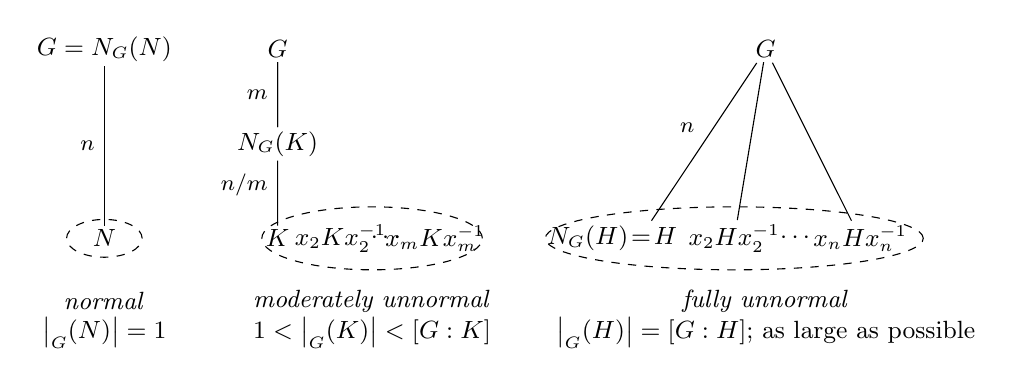
\begin{tikzpicture}[scale=.8]
    \tikzstyle{every node}=[font=\small]
    %%
    \begin{scope}[shift={(0,0)},shorten >= -2pt, shorten <= -2pt]
      \node (G) at (0,3) {$G=\Balert{N_G(N)}$};
      \node (N) at (0,0) {$N$};
      \draw (G)--(N) node[left,pos=.5] {\footnotesize $n$};
      \draw[dashed] (0,0) circle [x radius=.6cm, y radius=.3cm];
      \node at (0,-1) {\Balert{\emph{normal}}};
      \node at (0,-1.5) {$\big|\cl_G(N)\big|=1$};
    \end{scope}
    %%
    \begin{scope}[shift={(4.25,0)},shorten >= -2pt, shorten <= -2pt]
      \node (G) at (-1.5,3) {$G$};
      \node (N_G) at (-1.5,1.5) {\Palert{$N_G(K)$}};
      \node (K) at (-1.5,0) {$K$};
      \node (K2) at (-.5,0) {$x_2Kx_2^{-1}$};
      \node (K3) at (.25,0) {$\cdots$};
      \node (Kl) at (1,0) {$x_m Kx_m^{-1}$};
      \draw (G) -- (N_G);
      \draw (N_G) -- (K) node[left,pos=.35] {\footnotesize $n/m$};
      \draw (G)--(N_G) node[left,pos=.5] {\footnotesize $m$};
      \draw[dashed] (0,0) circle [x radius=1.75cm, y radius=.5cm];
      \node at (0,-1) {\Palert{\emph{moderately unnormal}}};
      \node at (0,-1.5) {$1<\big|\cl_G(K)\big|<[G:K]$};
    \end{scope}
    %%
    \begin{scope}[shift={(10.5,0)},shorten >= -2pt, shorten <= -2pt]
      \node (G) at (0,3) {$G$};
      \node (H) at (-2,0) {\hspace{-7mm}$\Alert{N_G(H)}\!=\!H$};
      \node (H2) at (-.5,0) {$x_2Hx_2^{-1}$};
      \node (H3) at (.5,0) {$\cdots$};
      \node (Hl) at (1.5,0) {$x_n Hx_n^{-1}$};
      \draw (G)--(H) node[above left,pos=.5] {\footnotesize $n$};
      \draw (G) -- (H2); \draw (G) -- (Hl);
      \draw[dashed] (-.5,0) circle [x radius=3cm, y radius=.5cm];
      \node at (0,-1) {\Alert{\emph{fully unnormal}}};
      \node at (0,-1.5) {$\big|\cl_G(H)\big|=[G:H]$; as large as possible};
    \end{scope}
  \end{tikzpicture}
  \]

\end{frame}

%%====================================================================

\begin{frame}{Groups acting on subgroups by conjugation}

  Here is an example of $G=D_3$ acting on its subgroups. \vspace{-2mm}

  %% Action graph of D_3 acting on its subgroups
  \[
  \begin{tikzpicture}[scale=.8]
    \tikzstyle{n} = [inner sep=1pt] 
    \tikzstyle{p} = [draw,bend left=30,-stealth]
    \tikzstyle{r-thin} = [draw, eRed, bend left=30, -stealth]
    \tikzstyle{b-thin} = [draw, eBlue, bend left=40, -stealth]
    \tikzstyle{every node}=[font=\small]
    %%
    \begin{scope}[shift={(0,5)}]
      \node [n] (0) at (0,0) {$\tau(1)\quad=\quad$};
      \node [n] (e) at (1,0) {$\<1\>$};
      \node [n] (r) at (2,0) {$\<r\>$};
      \node [n] (f) at (3,0) {$\<f\>$};
      \node [n] (rf) at (4,0) {$\<rf\>$};
      \node [n] (r2f) at (5,0) {$\<r^2f\>$};
      \node [n] (D3) at (6,0) {$D_3$};
    \end{scope}
    %%
    \begin{scope}[shift={(0,4)}]
      \node [n] (0) at (0,0) {\color{xRed} $\tau(r)\quad=\quad$};
      \node [n] (e) at (1,0) {\color{xRed} $\<1\>$};
      \node [n] (r) at (2,0) {\color{xRed} $\<r\>$};
      \node [n] (f) at (3,0) {\color{xRed} $\<f\>$};
      \node [n] (rf) at (4,0) {\color{xRed} $\<rf\>$};
      \node [n] (r2f) at (5,0) {\color{xRed} $\<r^2f\>$};
      \node [n] (D3) at (6,0) {$D_3$};
      \path [r-thin] (f) to (rf);
      \path [r-thin] (rf) to (r2f);
      \path [r-thin] (r2f) to (f);
    \end{scope}
    %%
    \begin{scope}[shift={(0,3)}]
      \node [n] (0) at (0,0) {$\tau(r^2)\quad=\quad$};
      \node [n] (e) at (1,0) {$\<1\>$};
      \node [n] (r) at (2,0) {$\<r\>$};
      \node [n] (f) at (3,0) {$\<f\>$};
      \node [n] (rf) at (4,0) {$\<rf\>$};
      \node [n] (r2f) at (5,0) {$\<r^2f\>$};
      \node [n] (D3) at (6,0) {$D_3$};
      \path [p] (rf) to (f);
      \path [p] (r2f) to (rf);
      \path [p] (f) to (r2f);
    \end{scope}
    %%
    \begin{scope}[shift={(0,2)}]
      \node [n] (0) at (0,0) {\color{xBlue} $\tau(f)\quad=\quad$};
      \node [n] (e) at (1,0) {\color{xBlue} $\<1\>$};
      \node [n] (r) at (2,0) {\color{xBlue} $\<r\>$};
      \node [n] (f) at (3,0) {\color{xBlue} $\<f\>$};
      \node [n] (rf) at (4,0) {\color{xBlue} $\<rf\>$};
      \node [n] (r2f) at (5,0) {\color{xBlue} $\<r^2f\>$};
      \node [n] (D3) at (6,0) {$D_3$};
      \path [b-thin] (rf) to (r2f);
      \path [b-thin] (r2f) to (rf);
    \end{scope}
    %%
    \begin{scope}[shift={(0,1)}]
      \node [n] (0) at (0,0) {$\tau(rf)\quad=\quad$};
      \node [n] (e) at (1,0) {$\<1\>$};
      \node [n] (r) at (2,0) {$\<r\>$};
      \node [n] (f) at (3,0) {$\<f\>$};
      \node [n] (rf) at (4,0) {$\<rf\>$};
      \node [n] (r2f) at (5,0) {$\<r^2f\>$};
      \node [n] (D3) at (6,0) {$D_3$};
      \path [p] (f) to (r2f);
      \path [p] (r2f) to (f);  
    \end{scope}
    %%
    \begin{scope}[shift={(0,0)}]
      \node [n] (0) at (0,0) {$\tau(r^2f)\quad=\quad$};
      \node [n] (e) at (1,0) {$\<1\>$};
      \node [n] (r) at (2,0) {$\<r\>$};
      \node [n] (f) at (3,0) {$\<f\>$};
      \node [n] (rf) at (4,0) {$\<rf\>$};
      \node [n] (r2f) at (5,0) {$\<r^2f\>$};
      \node [n] (D3) at (6,0) {$D_3$};
      \path [p] (f) to (rf);
      \path [p] (rf) to (f);
    \end{scope}
    %%
    \begin{scope}[shift={(9.5,-1.75)},shorten >= -3pt, shorten <= -3pt,
        yscale=1.1]
      \tikzstyle{every node}=[font=\small]
      %%
      \node(G) at (0,6) {$D_3$};
      \node(r) at (-1.75,4.5) {$\<r\>$};
      \node(1) at (0,1.5) {$\<1\>$};
      \node(f) at (.25,24/7) {$\<f\>$};
      \node(rf) at (1.75,24/7) {$\<rf\>$};
      \node(r2f) at (3.25,24/7) {$\<r^2\!f\>$};
      \draw[faded] (G)--(r); 
      \draw[faded] (G)--(f); 
      \draw[faded] (G)--(rf); 
      \draw[faded] (G)--(r2f); 
      \draw[faded] (r)--(1); 
      \draw[faded] (f)--(1);  
      \draw[faded] (rf)--(1); 
      \draw[faded] (r2f)--(1); 
      \draw [r] (f) to (rf);
      \draw [r] (rf) to (r2f);
      \draw [r] (r2f) to [bend left] (f);
      \draw [bb] (rf) to [bend left] (r2f);
      \path (G) edge [r,loop left,>=stealth] (G);
      \path (G) edge [b,loop right,>=stealth] (G);
      \path (r) edge [r,loop left,>=stealth] (r);
      \path (r) edge [b,loop right,>=stealth] (r);
      \path (1) edge [r,loop left,>=stealth] (1);
      \path (1) edge [b,loop right,>=stealth] (1);
      \path (f) edge [b,loop above,>=stealth] (f);
    \end{scope}
  \end{tikzpicture}
  \]
  
  \vspace{-2mm}
  
  \begin{exampleblock}{Observations}
    Do you see how to read stabilizers and fixed points off of the
    permutation diagram? \Pause
    \begin{itemize}
    \item \Balert{$\Ker(\phi)=\<1\>$} consists of the \Balert{row(s)}
      with only fixed points. \Pause
    \item \Galert{$\Fix(\phi)=\big\{\<1\>,\<r\>,D_3\big\}$} consists of the
      \Galert{column(s)} with only fixed points. \Pause
    \item By the orbit-counting theorem, there are
      $|\Alert{\Orb(\phi)}|=24/|D_3|=4$ conjugacy classes.
    \end{itemize}
  \end{exampleblock}
  
\end{frame}

%%====================================================================

\begin{frame}{Groups acting on subgroups by conjugation}
  
  Consider the partitions of $D_3$ by the left cosets of its six subgroups:
  %%
  %% Red/blue shoebox diagrams of the cosets of all 6 subgroups of D_3
  \[
  \begin{tikzpicture}[scale=.6]
    \tikzstyle{every node}=[font=\small]
    %%
    \begin{scope}[shift={(0,0)}]
      \draw[thin,fill=boxBlue] (0,0) rectangle (2,3);
      \node at (.5,2.5) {$r^2$}; \node at (1.5,2.5) {$r^2f$};
      \node at (.5,1.5) {$r$}; \node at (1.5,1.5) {$rf$};
      \node at (.5,.5) {$1$}; \node at (1.5,.5) {$f$};
      \node at (1,-.5) {$D_3/D_3$};
    \end{scope}
    %%
    \begin{scope}[shift={(2.75,0)}]
      \draw[thin,fill=boxBlue] (0,0) rectangle (1,3);
      \draw[thin,fill=boxBlue] (1,0) rectangle (2,3);
      \node at (.5,2.5) {$r^2$}; \node at (1.5,2.5) {$r^2f$};
      \node at (.5,1.5) {$r$}; \node at (1.5,1.5) {$rf$};
      \node at (.5,.5) {$1$}; \node at (1.5,.5) {$f$};
      \node at (1,-.5) {$D_3/\<r\>$};
    \end{scope}
    %%
    \begin{scope}[shift={(5.5,0)}]
      \draw[thin,fill=boxRed] (0,2) rectangle (2,3);
      \draw[thin,fill=boxRed] (0,1) rectangle (2,2);
      \draw[thin,fill=boxBlue] (0,0) rectangle (2,1);
      \node at (.5,2.5) {$r^2$}; \node at (1.5,2.5) {$r^2f$};
      \node at (.5,1.5) {$r$}; \node at (1.5,1.5) {$rf$};
      \node at (.5,.5) {$1$}; \node at (1.5,.5) {$f$};
      \node at (1,-.5) {$D_3/\<f\>$};
    \end{scope}
    %%
    \begin{scope}[shift={(8.25,0)}]
      \draw[thin,fill=boxRed] (0,2) rectangle (2,3);
      \draw[thin,fill=boxRed] (0,1) rectangle (2,2);
      \draw[thin,fill=boxBlue] (0,0) rectangle (2,1);
      \node at (.5,2.5) {$r^2$}; \node at (1.5,2.5) {$f$};
      \node at (.5,1.5) {$r$}; \node at (1.5,1.5) {$r^2f$};
      \node at (.5,.5) {$1$}; \node at (1.5,.5) {$rf$};
      \node at (1,-.5) {$D_3/\<rf\>$};
    \end{scope}
    %%
    \begin{scope}[shift={(11,0)}]
      \draw[thin,fill=boxRed] (0,2) rectangle (2,3);
      \draw[thin,fill=boxRed] (0,1) rectangle (2,2);
      \draw[thin,fill=boxBlue] (0,0) rectangle (2,1);
      \node at (.5,2.5) {$r^2$}; \node at (1.5,2.5) {$rf$};
      \node at (.5,1.5) {$r$}; \node at (1.5,1.5) {$f$};
      \node at (.5,.5) {$1$}; \node at (1.5,.5) {$r^2f$};
      \node at (1,-.5) {$D_3/\<r^2f\>$};
    \end{scope}
    %%
    \begin{scope}[shift={(13.75,0)}]
      \draw[thin,fill=boxBlue] (0,2) rectangle (2,3);
      \draw[thin,fill=boxBlue] (0,1) rectangle (2,2);
      \draw[thin,fill=boxBlue] (0,0) rectangle (2,1);
      \draw[thin] (1,0) to (1,3);
      \node at (.5,2.5) {$r^2$}; \node at (1.5,2.5) {$r^2f$};
      \node at (.5,1.5) {$r$}; \node at (1.5,1.5) {$rf$};
      \node at (.5,.5) {$1$}; \node at (1.5,.5) {$f$};
      \node at (1,-.5) {$D_3/\<1\>$};
    \end{scope}
  \end{tikzpicture}
  \]
  
  \begin{itemize}
  \item $\fix(g)$ are the subgroups $H$ for which ``\emph{$g$ appears
    in a blue coset of $H$}'' \smallskip
  \item $\Ker(\phi)$ are elements that ``\emph{only appear in blue
    cosets}'' \smallskip
  \item By the orbit-counting theorem, the subgroups fall into
    \[
    |\Orb(\phi)|=\text{average \# checkmarks per row}
    =\frac{\text{total \# of blue entries}}{|G|}
    \]
    conjugacy classes. \medskip
    
    Equivalently: \emph{how many full ``$G$-boxes'' the
      blue cosets can be rearranged to fill up.}
  \end{itemize}
  
\end{frame}

%%====================================================================

\begin{frame}{Groups acting on subgroups by conjugation}

  Here is an example of
  $G=A_4=\<{\color{xRed}(123)},{\color{xBlue}(12)(34)}\>$ acting on its
  subgroups.

  %% Action graph of A_4 acting on its subgroups by conjugation
  \[
  \begin{tikzpicture}[shorten >= -3pt, shorten <= -3pt,auto]
    \tikzstyle{every node}=[font=\normalsize]
    %%
    \begin{scope}[shift={(0,0)},scale=.9]
      \node(A4) at (0,6) {$A_4$};
      \node(V4) at (2.25,4) {$\big\<(12)(34),(13)(24)\big\>$};
      \node(C34) at (-.75,3) {$\big\<(234)\big\>$};
      \node(C33) at (-2.25,3){$\big\<(134)\big\>$};
      \node(C32) at (-3.75,3){$\big\<(124)\big\>$};
      \node(C31) at (-5.25,3) {$\big\<(123)\big\>$};
      \node(C21) at (.75,2) {$\big\<(12)(34))\big\>$};
      \node(C22) at (2.75,2) {$\big\<(13)(24)\big\>$};
      \node(C23) at (4.75,2) {$\big\<(14)(23))\big\>$};
      \node(1) at (0,0) {$\<e\>$};
      \draw[faded] (A4)--(V4);
      \draw[faded] (A4)--(C31);
      \draw[faded] (A4)--(C32);
      \draw[faded] (A4)--(C33);
      \draw[faded] (A4)--(C34);
      \draw[faded] (C31)--(1);
      \draw[faded] (C32)--(1);
      \draw[faded] (C33)--(1);
      \draw[faded] (C34)--(1);
      \draw[faded] (V4)--(C21);
      \draw[faded] (V4)--(C22);
      \draw[faded] (V4)--(C23);
      \draw[faded] (C21)--(1);
      \draw[faded] (C22)--(1);
      \draw[faded] (C23)--(1);
      \path (A4) edge [r,loop left,>=stealth] (A4);
      \path (A4) edge [b,loop right,>=stealth] (A4);
      \path (V4) edge [r,loop above,>=stealth] (V4);
      \path (V4) edge [b,loop below,>=stealth] (V4);
      \path (C31) edge [r,loop above,>=stealth] (C31); 
      \draw [r] (C33) to[bend right=40] (C32);
      \draw [r] (C34) to[bend right=40] (C33);
      \draw [r] (C32) to[bend right=30] (C34);      
      \draw [bb] (C31) to (C32);
      \draw [bb] (C33) to (C34);
      \path (C21) edge [b,loop above,>=stealth] (C21);
      \path (C22) edge [b,loop above,>=stealth] (C22);
      \path (C23) edge [b,loop above,>=stealth] (C23);
      \path (1) edge [r,loop left,>=stealth] (1);
      \path (1) edge [b,loop right,>=stealth] (1);
      \draw [r] (C22) to[bend right=35] (C21);
      \draw [r] (C23) to[bend right=35] (C22);
      \draw [r] (C21) to[bend right=25] (C23);
    \end{scope}
  \end{tikzpicture}
  \]
  
  Let's take a moment to revisit our ``\emph{three favorite examples}''
  from Chapter 3.
  \[
  N=\big\<(12)(34),(13)(24)\big\>,\qquad H=\big\<(123)\big\>,\qquad K
  =\big\<(12)(34)\big\>.
  \]
  
\end{frame}

%%====================================================================

\begin{frame}{Groups acting on subgroups by conjugation}
  
  Here is the ``\emph{fixed point table}'' of the action of $A_4$ on
  its subgroups.
  \[
  \hspace{-5mm}
  \scalebox{.77}{
    \begin{tikzpicture}
      \node at (0,0) {
        \renewcommand\arraystretch{1.7}
        \begin{tabular}{c|cccccccccc}
          & {\small$\<e\>$} & {\small$\<(123)\>$} & {\small$\<(124)\>$} & {\small$\<(134)\>$} & {\small$\<(234)\>$} & {\small$\<(12)(34)\>$} & {\small$\<(13)(24)\>$} & {\small$\<(14)(23)\>$} & {\small$\<(12)(34),(13)(24)\>$} & {\small $A_4$} \\ \hline
          \small $e$ & \checkmark & \checkmark & \checkmark & \checkmark & \checkmark & \checkmark & \checkmark & \checkmark & \checkmark & \checkmark \\
\small $(123)$ & \checkmark & \checkmark & & & & & & & \checkmark & \checkmark \\
\small $(132)$ & \checkmark & \checkmark & & & & & & & \checkmark & \checkmark \\
\small $(124)$ & \checkmark & & \checkmark & & & & & & \checkmark & \checkmark \\
\small $(142)$ & \checkmark & & \checkmark & & & & & & \checkmark & \checkmark \\
\small $(134)$ & \checkmark & & & \checkmark & & & & & \checkmark & \checkmark \\
\small $(143)$ & \checkmark & & & \checkmark & & & & & \checkmark & \checkmark \\
\small $(234)$ & \checkmark & & & & \checkmark & & & & \checkmark & \checkmark \\
\small $(243)$ & \checkmark & & & & \checkmark & & & & \checkmark & \checkmark \\
\small $(12)(34)$ & \checkmark & & & & & \checkmark & \checkmark & \checkmark & \checkmark & \checkmark \\
\small $(13)(24)$ & \checkmark & & & & & \checkmark & \checkmark & \checkmark & \checkmark & \checkmark \\
\small $(14)(23)$ & \checkmark & & & & & \checkmark & \checkmark & \checkmark & \checkmark & \checkmark \\
      \end{tabular}};
  \end{tikzpicture}}
  \]
  
  \Pause
  
  By the \textbf{orbit-counting theorem}, there are 
  $|\Orb(\phi)|=60/|A_4|=5$ conjugacy classes. 
  
\end{frame}

%%====================================================================

\begin{frame}{Groups acting on cosets of $H$ by multiplication} %\Pause
  
  Fix a subgroup $H\leq G$. Then $G$ acts on its \textbf{right cosets}
  by \textbf{right-multiplication}:
  \[
  \phi\colon G\longto\Perm(S)\,,\qquad
  \phi(g)=\mbox{\footnotesize the permutation that sends each $Hx$ to
    $Hxg$.}
  \]
  
  \Pause
  
  Let $Hx$ be an element of $S=H\!\setminus\!G$ (the right cosets of
  $H$). \Pause
  \begin{itemize}
  \item There is \Alert{only one orbit}. \Pause For example, given two cosets
    $Hx$ and $Hy$,
    \[
    \text{$\phi(x^{-1}y)$\; sends\; $Hx\longmapsto Hx(x^{-1}y)=Hy$}.
    \]   
    \vspace{-4mm}\Pause
  \item The \Balert{stabilizer} of $Hx$ is the
    \Balert{conjugate subgroup} $x^{-1}Hx$: 
    \[
    \stab(Hx)=\big\{g\in G\mid Hxg=Hx\big\}\Pause=\big\{g\in G\mid
    Hxgx^{-1}=H\big\} \Pause=x^{-1}Hx.
    \]
    \vspace{-4mm}\Pause    
  \item There doesn't seem to be a standard term for the
    \Galert{fixator} of $g$:
    \[
    \fix(g)=\big\{Hx\mid Hxg=Hx\big\}=\big\{Hx\mid xgx^{-1}\in H\big\}.
    \]
    \vspace{-4mm}\Pause
  \item Assuming $H\neq G$, there are {\color{xGreen}no fixed
    points} of $\phi$. 

    \smallskip\Pause
    
  \item The \Balert{kernel} of this action is the intersection of all
    conjugate subgroups of $H$:
    \[
    \Ker(\phi)=\bigcap_{x\in G}\stab(x)=\bigcap_{x\in G}x^{-1}Hx.
    \]
    \Pause Notice that $\<1\>\leq\Ker\phi\leq H$, and $\Ker(\phi)=H$ iff
    $H\normaleq G$.
  \end{itemize}
  
\end{frame}

%%====================================================================

\begin{frame}{Groups acting on cosets of $H$ by multiplication} %\Pause
  
  The quotient process is done by collapsing the Cayley graph by the
  \Alert{left cosets} of $H$.
  
  \bigskip\Pause
  
  In contrast, this action is the result of collapsing the Cayley
  graph by the \Alert{right cosets}.
  
  %% Collapsing left vs. right cosets of H=<f> in D_6
  \[
  \begin{tikzpicture}[scale=.45, auto]
    \tikzstyle{v} = [circle, draw, fill=lightgray,inner sep=0pt,
      minimum size=3.75mm] 
    \tikzstyle{rFaded} = [draw, thick, fRed]
    \tikzstyle{r-thick} = [draw, eRed, very thick, -stealth', shorten >= 6pt,
      shorten <= 6pt,bend right=15]
    \tikzstyle{rr-thick} = [draw, eRed, very thick, shorten >= 6pt,
      shorten <= 6pt,bend right=15]
    \tikzstyle{every node}=[font=\small]
    %%
    \begin{scope}[shift={(0,0)}]
      \draw[eBlue, fill=cosetBlue,rotate=90] (0,2.3) circle (.7);
      \draw[eBlue, fill=cosetBlue,rotate=90] (0,4.7) circle (.7);
      \draw[cosetBlue, fill=cosetBlue,rotate=90] (-.7,2.3) rectangle (.7,4.7);
      \draw[eBlue,rotate=90] (-.7,2.3) to (-.7,4.7);
      \draw[eBlue,rotate=90] (.7,2.3) to (.7,4.7);
      %%
      \draw[eRed, fill=cosetRed, rotate=30] (0,2.3) circle (.7);
      \draw[eRed, fill=cosetRed, rotate=30] (0,4.7) circle (.7);
      \draw[cosetRed, fill=cosetRed, rotate=30] (-.7,2.3) rectangle (.7,4.7);
      \draw[eRed,rotate=30] (-.7,2.3) to (-.7,4.7);
      \draw[eRed,rotate=30] (.7,2.3) to (.7,4.7);
      %%
      \draw[eRed, fill=cosetRed, rotate=150] (0,2.3) circle (.7);
      \draw[eRed, fill=cosetRed, rotate=150] (0,4.7) circle (.7);
      \draw[cosetRed, fill=cosetRed, rotate=150] (-.7,2.3) rectangle (.7,4.7);
      \draw[eRed,rotate=150] (-.7,2.3) to (-.7,4.7);
      \draw[eRed,rotate=150] (.7,2.3) to (.7,4.7);
      %%
      \draw[eBlue, fill=cosetBlue, rotate=-90] (0,2.3) circle (.7);
      \draw[eBlue, fill=cosetBlue, rotate=-90] (0,4.7) circle (.7);
      \draw[cosetBlue, fill=cosetBlue, rotate=-90] (-.7,2.3) rectangle (.7,4.7);
      \draw[eBlue,rotate=-90] (-.7,2.3) to (-.7,4.7);
      \draw[eBlue,rotate=-90] (.7,2.3) to (.7,4.7);
      %%
      \draw[eRed, fill=cosetRed, rotate=210] (0,2.3) circle (.7);
      \draw[eRed, fill=cosetRed, rotate=210] (0,4.7) circle (.7);
      \draw[cosetRed, fill=cosetRed, rotate=210] (-.7,2.3) rectangle (.7,4.7);
      \draw[eRed,rotate=210] (-.7,2.3) to (-.7,4.7);
      \draw[eRed,rotate=210] (.7,2.3) to (.7,4.7);
      %%
      \draw[eRed, fill=cosetRed, rotate=330] (0,2.3) circle (.7);
      \draw[eRed, fill=cosetRed, rotate=330] (0,4.7) circle (.7);
      \draw[cosetRed, fill=cosetRed, rotate=330] (-.7,2.3) rectangle (.7,4.7);
      \draw[eRed,rotate=330] (-.7,2.3) to (-.7,4.7);
      \draw[eRed,rotate=330] (.7,2.3) to (.7,4.7);
      %%
      \node (v0) at (0:3.75) {};
      \node (v1) at (60:3.75) {};
      \node (v2) at (120:3.75) {};
      \node (v3) at (180:3.75) {};
      \node (v4) at (240:3.75) {};
      \node (v5) at (300:3.75) {};
      \node (1) at (0:4.5) [v] {$1$};
      \node (r) at (60:4.5) [v] {$r$};
      \node (r2) at (120:4.5) [v] {$r^2$};
      \node (r3) at (180:4.5) [v] {$r^3$};
      \node (r4) at (240:4.5) [v] {$r^4$};
      \node (r5) at (300:4.5) [v] {$r^5$};
      \node (f) at (0:2.5) [v] {$f$};
      \node (fr) at (60:2.5) [v] {$rf$};
      \node (fr2) at (120:2.5) [v] {$r^2\!f$};
      \node (fr3) at (180:2.5) [v] {$r^3\!f$};
      \node (fr4) at (240:2.5) [v] {$r^4\!f$};
      \node (fr5) at (300:2.5) [v] {$r^5\!f$};
      %%
      \path[bbFaded] (1) to (f);
      \path[bbFaded] (r) to (fr);
      \path[bbFaded] (r2) to (fr2);
      \path[bbFaded] (r3) to (fr3);
      \path[bbFaded] (r4) to (fr4);
      \path[bbFaded] (r5) to (fr5);
      \draw [rr-thick] (v0) to (v1);
      \draw [rr-thick] (v1) to (v2);
      \draw [rr-thick] (v2) to (v3);
      \draw [rr-thick] (v3) to (v4);
      \draw [rr-thick] (v4) to (v5);
      \draw [rr-thick] (v5) to (v0);
      \node at (-15:5.5) {\normalsize $\bm{H}$};
      \node at (45:5.5) {\normalsize $\bm{rH}$};
      \node at (135:5.5) {\normalsize $\bm{r^2H}$};
      \node at (195:5.5) {\normalsize $\bm{r^3H}$};
      \node at (225:5.5) {\normalsize $\bm{r^4H}$};
      \node at (315:5.5) {\normalsize $\bm{r^5H}$};
      \node at (270:6.5) {\normalsize \emph{not a valid action graph}};
    \end{scope}
    %%
    \begin{scope}[shift={(13,0)}]
      \draw[eBlue, fill=cosetBlue,rotate=90] (0,2.3) circle (.7);
      \draw[eBlue, fill=cosetBlue,rotate=90] (0,4.7) circle (.7);
      \draw[cosetBlue, fill=cosetBlue,rotate=90] (-.7,2.3) rectangle (.7,4.7);
      \draw[eBlue,rotate=90] (-.7,2.3) to (-.7,4.7);
      \draw[eBlue,rotate=90] (.7,2.3) to (.7,4.7);
      %%
      \draw[eRed, fill=cosetRed, rotate=30] (0,2.3) circle (.7);
      \draw[eRed, fill=cosetRed, rotate=30] (0,4.7) circle (.7);
      \draw[cosetRed, fill=cosetRed, rotate=30] (-.7,2.3) rectangle (.7,4.7);
      \draw[eRed,rotate=30] (-.7,2.3) to (-.7,4.7);
      \draw[eRed,rotate=30] (.7,2.3) to (.7,4.7);
      %%
      \draw[eRed, fill=cosetRed, rotate=150] (0,2.3) circle (.7);
      \draw[eRed, fill=cosetRed, rotate=150] (0,4.7) circle (.7);
      \draw[cosetRed, fill=cosetRed, rotate=150] (-.7,2.3) rectangle (.7,4.7);
      \draw[eRed,rotate=150] (-.7,2.3) to (-.7,4.7);
      \draw[eRed,rotate=150] (.7,2.3) to (.7,4.7);
      %%
      \draw[eBlue, fill=cosetBlue, rotate=-90] (0,2.3) circle (.7);
      \draw[eBlue, fill=cosetBlue, rotate=-90] (0,4.7) circle (.7);
      \draw[cosetBlue, fill=cosetBlue, rotate=-90] (-.7,2.3) rectangle (.7,4.7);
      \draw[eBlue,rotate=-90] (-.7,2.3) to (-.7,4.7);
      \draw[eBlue,rotate=-90] (.7,2.3) to (.7,4.7);
      %%
      \draw[eRed, fill=cosetRed, rotate=210] (0,2.3) circle (.7);
      \draw[eRed, fill=cosetRed, rotate=210] (0,4.7) circle (.7);
      \draw[cosetRed, fill=cosetRed, rotate=210] (-.7,2.3) rectangle (.7,4.7);
      \draw[eRed,rotate=210] (-.7,2.3) to (-.7,4.7);
      \draw[eRed,rotate=210] (.7,2.3) to (.7,4.7);
      %%
      \draw[eRed, fill=cosetRed, rotate=330] (0,2.3) circle (.7);
      \draw[eRed, fill=cosetRed, rotate=330] (0,4.7) circle (.7);
      \draw[cosetRed, fill=cosetRed, rotate=330] (-.7,2.3) rectangle (.7,4.7);
      \draw[eRed,rotate=330] (-.7,2.3) to (-.7,4.7);
      \draw[eRed,rotate=330] (.7,2.3) to (.7,4.7);
      \node (v0) at (0:3.75) {};
      \node (v1) at (60:3.75) {};
      \node (v2) at (120:3.75) {};
      \node (v3) at (180:3.75) {};
      \node (v4) at (240:3.75) {};
      \node (v5) at (300:3.75) {};
      \node (u1) at (60:1.6) {};
      \node (u2) at (120:1.6) {};
      \node (u4) at (240:1.6) {};
      \node (u5) at (300:1.6) {};
      \node (1) at (0:4.5) [v] {$1$};
      \node (r) at (60:4.5) [v] {$r$};
      \node (r2) at (120:4.5) [v] {$r^2$};
      \node (r3) at (180:4.5) [v] {$r^3$};
      \node (r4) at (240:4.5) [v] {$r^4$};
      \node (r5) at (300:4.5) [v] {$r^5$};
      \node (f) at (0:2.5) [v] {$f$};
      \node (fr) at (60:2.5) [v] {$fr$};
      \node (fr2) at (120:2.5) [v] {$fr^2$};
      \node (fr3) at (180:2.5) [v] {$fr^3$};
      \node (fr4) at (240:2.5) [v] {$fr^4$};
      \node (fr5) at (300:2.5) [v] {$fr^5$};
      \path[bbFaded] (1) to (f);
      \path[bbFaded] (r3) to (fr3);
      \path[bb,shorten >= -3.5pt, shorten <= -3.5pt] (u1) to (u5);
      \path[bb,shorten >= -3.5pt, shorten <= -3.5pt] (u2) to (u4);
      \draw [r-thick] (v0) to (v1);
      \draw [r-thick] (v1) to (v2);
      \draw [r-thick] (v2) to (v3);
      \draw [r-thick] (v3) to (v4);
      \draw [r-thick] (v4) to (v5);
      \draw [r-thick] (v5) to (v0);
      \tikzset{every loop/.style={min distance=20mm,in=60,out=120,looseness=40}}
      \path (-4.5,.7) edge [b,loop above,>=stealth] (-4.5,.7);
      \path (4.5,.7) edge [b,loop above,>=stealth] (-4.5,.7);
      \node at (-15:5.5) {\normalsize $\bm{H}$};
      \node at (45:5.5) {\normalsize $\bm{Hr}$};
      \node at (135:5.5) {\normalsize $\bm{Hr^2}$};
      \node at (195:5.5) {\normalsize $\bm{Hr^3}$};
      \node at (225:5.5) {\normalsize $\bm{Hr^4}$};
      \node at (315:5.5) {\normalsize $\bm{Hr^5}$};
      \node at (270:6.5) {\normalsize \emph{action graph of $\phi$}};
    \end{scope}
  \end{tikzpicture}
  \]
  
\end{frame}

%%====================================================================

\begin{frame}{Subgroups of small index}

  Groups acting on cosets is a useful technique for establishing
  seemingly unrelated results. \medskip\Pause

  Several of these involving showing that subgroups of ``small index''
  are normal. \medskip\Pause

  We've already seen that subgroups of index $2$ are normal. \medskip\Pause

  Of course, there are non-normal index-$3$ subgroups, like $\<f\>\leq
  D_3$. \medskip\Pause

  The following gives a sufficient condition for when index-$3$
  subgroups are normal.
  
  \smallskip\Pause
  
  \begin{block}{Proposition}
    If $G$ has no subgroup of index $2$, then any subgroup of index
    $3$ is normal.
  \end{block}
  
  \begin{exampleblock}{Proof} \Pause
    Let $H\leq G$ with $[G:H]=3$. \medskip\Pause
    
    Let $G$ act on the cosets of $H$ by multiplication, to get a
    nontrivial homomorphism
    \[
    \phi\colon G\longto S_3.
    \]
    \Pause $K:=\Ker(\phi)\leq H$ is the largest normal
    subgroup of $G$ contained in $H$. \Pause By the FHT,
    \[
    G/K\cong\Image(\phi)\leq S_3. 
    \]
  \end{exampleblock}
  
\end{frame}

%%====================================================================

\begin{frame}{Subgroups of small index}
  
  \begin{exampleblock}{Proof (contin.)}
    Thus, there are three cases for this quotient:
    \[
    G/K\cong S_3,\qquad G/K\cong C_3,\qquad G/K\cong C_2.
    \]   
    \Pause Visually, this means that we have one of the following:
    %%
    %% Possible subgroup lattices of G/K:  S_3, C_3, and C_2
    \[
    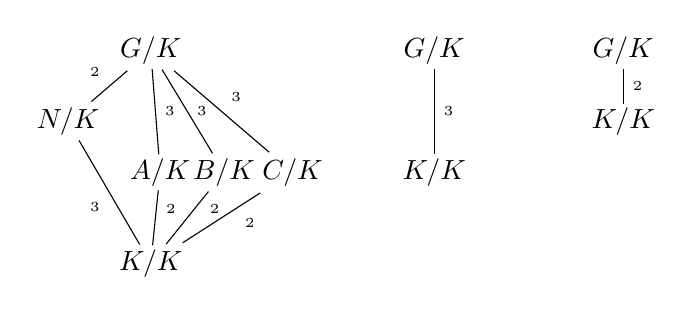
\begin{tikzpicture}[shorten >= -2pt,shorten <= -2pt,scale=.6]
      \begin{scope}[shift={(0,0)},scale=1]
        \node(G) at (0,6) {$G/K$};
        \node(N) at (-1.75,4.5) {$N/K$};
        \node(K) at (0,1.5) {$K/K$};
        \node(H1) at (.2,24/7) {$A/K$};
        \node(H2) at (1.55,24/7) {$B/K$};
        \node(H3) at (3,24/7) {$C/K$};
        \draw(N)--(K) node[midway, below left]{\tiny $3$};
        \draw(G)--(H1) node[midway,right]{\tiny $3$};
        \draw(G)--(H2) node[midway,right]{\tiny $3$};
        \draw(G)--(H3) node[midway,above right]{\tiny $3$};
        \draw(G)--(N) node[midway,above left]{\tiny $2$};
        \draw(K)--(H1) node[pos=.7,right]{\tiny $2$};
        \draw(K)--(H2) node[pos=.7,right]{\tiny $\;2$};
        \draw(K)--(H3) node[pos=.7,below right]{\tiny $2$};
      \end{scope}
      %%
      \begin{scope}[shift={(6,0)},scale=1]
        \node(G) at (0,6) {$G/K$};
        \node(K) at (0,24/7) {$K/K$};
        \draw(G)--(K) node[midway,right]{\tiny $3$};
      \end{scope}
      %%
      \begin{scope}[shift={(10,0)},scale=1]
        \node(G) at (0,6) {$G/K$};
        \node(K) at (0,4.5) {$K/K$};
        \draw(G)--(K) node[midway,right]{\tiny $2$};
      \end{scope}
    \end{tikzpicture}
    \]
    \pause By the corrdespondence theorem, $K\leq H\lneq G$ implies $K/K\leq
    H/K\lneq G/K$. \medskip\Pause
    
    Since $G$ has no index-$2$ subgroup, only the middle case is
    possible (\emph{Why?}). \medskip\Pause
    
    This forces $K/K=H/K$, and so $K=H$ which is normal for multiple
    reasons. $\hfill\Box$ 
  \end{exampleblock}
  
\end{frame}

%%====================================================================

\begin{frame}{Subgroups of small index}

  \begin{block}{Proposition}
    Suppose $H\leq G$ and $[G:H]=p$, the smallest prime dividing
    $|G|$. Then $H\normaleq G$.
  \end{block}

  \begin{exampleblock}{Proof} \Pause
    Let $G$ act on the cosets of $H$ by multiplication, to get a
    non-trivial homomorphism
    \[
    \phi\colon G\longto S_p.
    \]
    \Pause The kernel $K=\Ker(\phi)$, is the largest normal subgroup of $G$
    such that $K\leq H\lneq G$. \medskip\Pause

    We'll show that $H=K$, or equivalently, that $[H:K]=1$. \Pause
    By the correspondence theorem:
    %%
    %% Subgroups K < H < G, and K/K < H/K < G/K.
    \[
    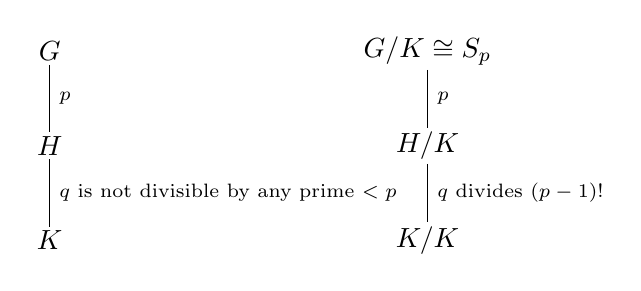
\begin{tikzpicture}[shorten >= -2pt,shorten <= -2pt,scale=.6]
      \begin{scope}[shift={(0,0)},scale=2]
        \node(G) at (0,2) {$G$};
        \node(H) at (0,1) {$H$};
        \node(K) at (0,0) {$K$};
        \draw(G)--(H) node[midway,right] {\scriptsize $p$};
        \draw(H)--(K) node[midway,right]
             {\scriptsize $q$ is not divisible by any prime $<p$};
      \end{scope}
      %%
      \begin{scope}[shift={(8,0)},scale=2]
        \node(G) at (0,2) {$G/K\cong S_p$};
        \node(H) at (0,1) {$H/K$};
        \node(K) at (0,0) {$K/K$};
        \draw(G)--(H) node[midway,right]{\scriptsize $p$};
        \draw(H)--(K) node[midway,right]{\scriptsize $q$ divides $(p-1)!$};
      \end{scope}
    \end{tikzpicture}
    \]
    \vspace{-6mm}
    
    Do you see why $q=1$? $\hfill\Box$
  \end{exampleblock}
  
\end{frame}

%%====================================================================

\begin{frame}{A summary of our four actions}
  
  Thus far, we have seen four important (right) actions of a group $G$, acting:

  \begin{itemize}
  \item on itself by multiplication
  \item on itself by conjugation. 
  \item on its subgroups by conjugation. 
  \item on the cosets of a fixed subgroup $H\leq G$ by
    multiplication. \Pause
  \end{itemize}
  
  \bigskip  
  \scalebox{.95}{  
    \def\arraystretch{1.75}
    \begin{tabular}{|c|cccc|} \hline
      set $S=$ & \multicolumn{2}{c}{$G$} & subgroups of $G$ & right cosets of $H$ \\ \hline
      operation & multiplication & conjugation  & conjugation &  right multiplication \\ \hline
      $\orb(s)$ & $G$ & $\cl_G(g)$ & $\cl_G(H)$ & all right cosets \\
      $\stab(s)$ & $\<1\>$ & $C_G(g)$ & $N_G(H)$ & $x^{-1}Hx$ \\
      $\fix(g)$ & $G$ or $\emptyset$ & $C_G(g)$ & $\{H\mid g\in N_G(H)\}$ & $\big\{Hx\mid xgx^{-1}\in H\big\}$ \\
      $\Ker(\phi)$ & $\<1\>$ & $Z(G)$ & $\displaystyle\bigcap_{H\leq G} N_G(H)$ &
      largest norm. subgp. $N\leq H$ \\
      $\Fix(\phi)$ & $\emptyset$ & $Z(G)$ & normal subgroups & none \\ \hline
  \end{tabular}}
  
\end{frame}


%%====================================================================

\section{The end!}
%%====================================================================

\end{document}